\label{sec:SignalRegDef}

The definitions of the signal regions have been studied to provide an optimal performance for $\sqrt s=13$ TeV collisions and a low integrated luminosity (2-4~\ifb). 
This optimization process was first performed with DC14 MC samples, and was then refined with the more accurate MC15 samples and close-to-final object definitions. 
We chose to categorize the signal regions based on their $b$-jet multiplicity, in continuation of the approach sustained in the Run-1 analysis: 
\begin{itemize}
\item[$\bullet$] Signal region(s) with at least one $b$-jet (``SR1b''): these selections target signal scenarios involving top or bottom quarks, 
mostly related to third-generation squarks, such as the benchmark process $\sbot\sbot^*\to t\bar t\tilde\chi_1^+\tilde\chi_1^-$. 
\item[$\bullet$] Signal region(s) with at least three $b$-jets (``SR3b''): these selections target signal scenarios involving many top or bottom quarks, 
such as the benchmark process $\gluino\gluino\to t\bar tt\bar t\ninoone\ninoone$, 
and with their intrinsically very low background are particularly well suited for scenarios with compressed mass spectra. 
\item[$\bullet$] Signal region(s) with a $b$-jet veto (``SR0b''): these selections allow to increase the sensitivity to signal scenarios without bottom quarks, 
by suppressing most of the top background -- the selections are then dominated by diboson background. 
\end{itemize}
One can notice that there is no dedicated selection for final states with $\ge 2$ $b$-jets: 
it is found to not be particularly useful, as the background is generally dominated by $t\bar t+X$ processes, 
which does not change substantially between $\ge 1$ and $\ge 2$ $b$-jets selections. 
By contrast the difference between $\ge 1$ and $\ge 3$ $b$-jets selections is very important. 

To this first classification we add minimal requirements on the inclusive jet multiplicity: 
\begin{center}
\begin{tabular}{c|c|c|c|c}
Signal region(s) & \multicolumn{2}{c|}{SR0b} & SR1b & SR3b\\\hline
Jets req. & $\ge 3$ ($p_T>50$~GeV) & $\ge 5$ ($p_T>50$~GeV) & $\ge 4$ ($p_T>50$~GeV) & $-$\\
\end{tabular}
\end{center}
As one can see, the SR0b selections were subdivided into two overlapping selections ($\ge 3$ or $\ge 5$ jets, 
also denoted as SR0b5j and SR0b3j) to cover various signal scenarios that lead to differently jet-enriched final states. 
The optimal minimal number of jets and the jet $p_T$ thresholds were defined as part of the DC14-based optimization, through a (\meff, \met, \#jets, jet $p_T$) scan similar to the one described below 
and focused on the few benchmark signal scenarios that were produced for DC14 studies. Only the $\pt$ threshold for SR0b3j was raised from 40 to 50~GeV for homogenization among the SRs since this change had very small impact in the sensitivity.

All these selections are inclusive in terms of leptons (``at least two same-sign leptons''), 
it was found that for these early results no substantial gain would be achieved by considering trilepton final states separately (as was done in the Run-1 analysis) except for SR0b3j, where a $\geq$3 lepton requirement was found to improve the sensitivity to slepton-mediated signals ($\gluino\to q\bar{q}(\ell\ell/\ell\nu)\ninoone$).

To complete the definition of the signal regions, we added requirements on the effective mass \meff{} and missing transverse momentum \met. 
We rely only on these two discriminant variables, well suited for generic SUSY searches, 
as one of the analysis strengths is to be sensitive to a broad range of BSM scenarios and we do not want to overtune it to a restricted set of benchmarks. 

\subsection{Optimization procedure and results}

The optimization of the signal region definitions was carried on with the MC15 samples. % (resp. the 50/25 ns configuration for background/signal). 
We scanned the $(\meff,\met)$ plane for the four selections detailed above, 
looking at the impact of the cuts on various signal benchmarks. 
We used as figure of merit the signal discovery significance (Zn), calculated with {\tt RooStats::NumberCountingUtils::BinominalObsZ} 
assuming an overall $40\%$ systematic uncertainty on the background prediction (as a compromise to the 50\% expected uncertainty on the fake-lepton background and 30\% on the prompt-lepton background). 
We discarded the cut configurations where the background projection was too imprecise, due to limited MC statistics; 
more precisely when the statistical error on the projected background exceeded $30\%$. 
We also focused on signal benchmarks that would provide at least 2 signal events for the considered luminosity. 

Figure~\ref{fig:OptimScan} shows as an example the $(\meff, \met)$ planes for two different signal regions and models.
The resulting maximum discovery significance across the signal grids and the corresponding $(\meff,\met)$ configurations 
are shown in Figure~\ref{fig:OptimSig1} for SR1b, SR3b and SR0b5j. As shown, with 2~\ifb\ of data we can have sensitivity beyond the existing Run-1 limits in some of the models. Note that the Run-1 limits shown in the figures correspond to the best ATLAS limit, not necessarily obtained by the SS/3L analysis.

\begin{figure}[!htb]
\centering
  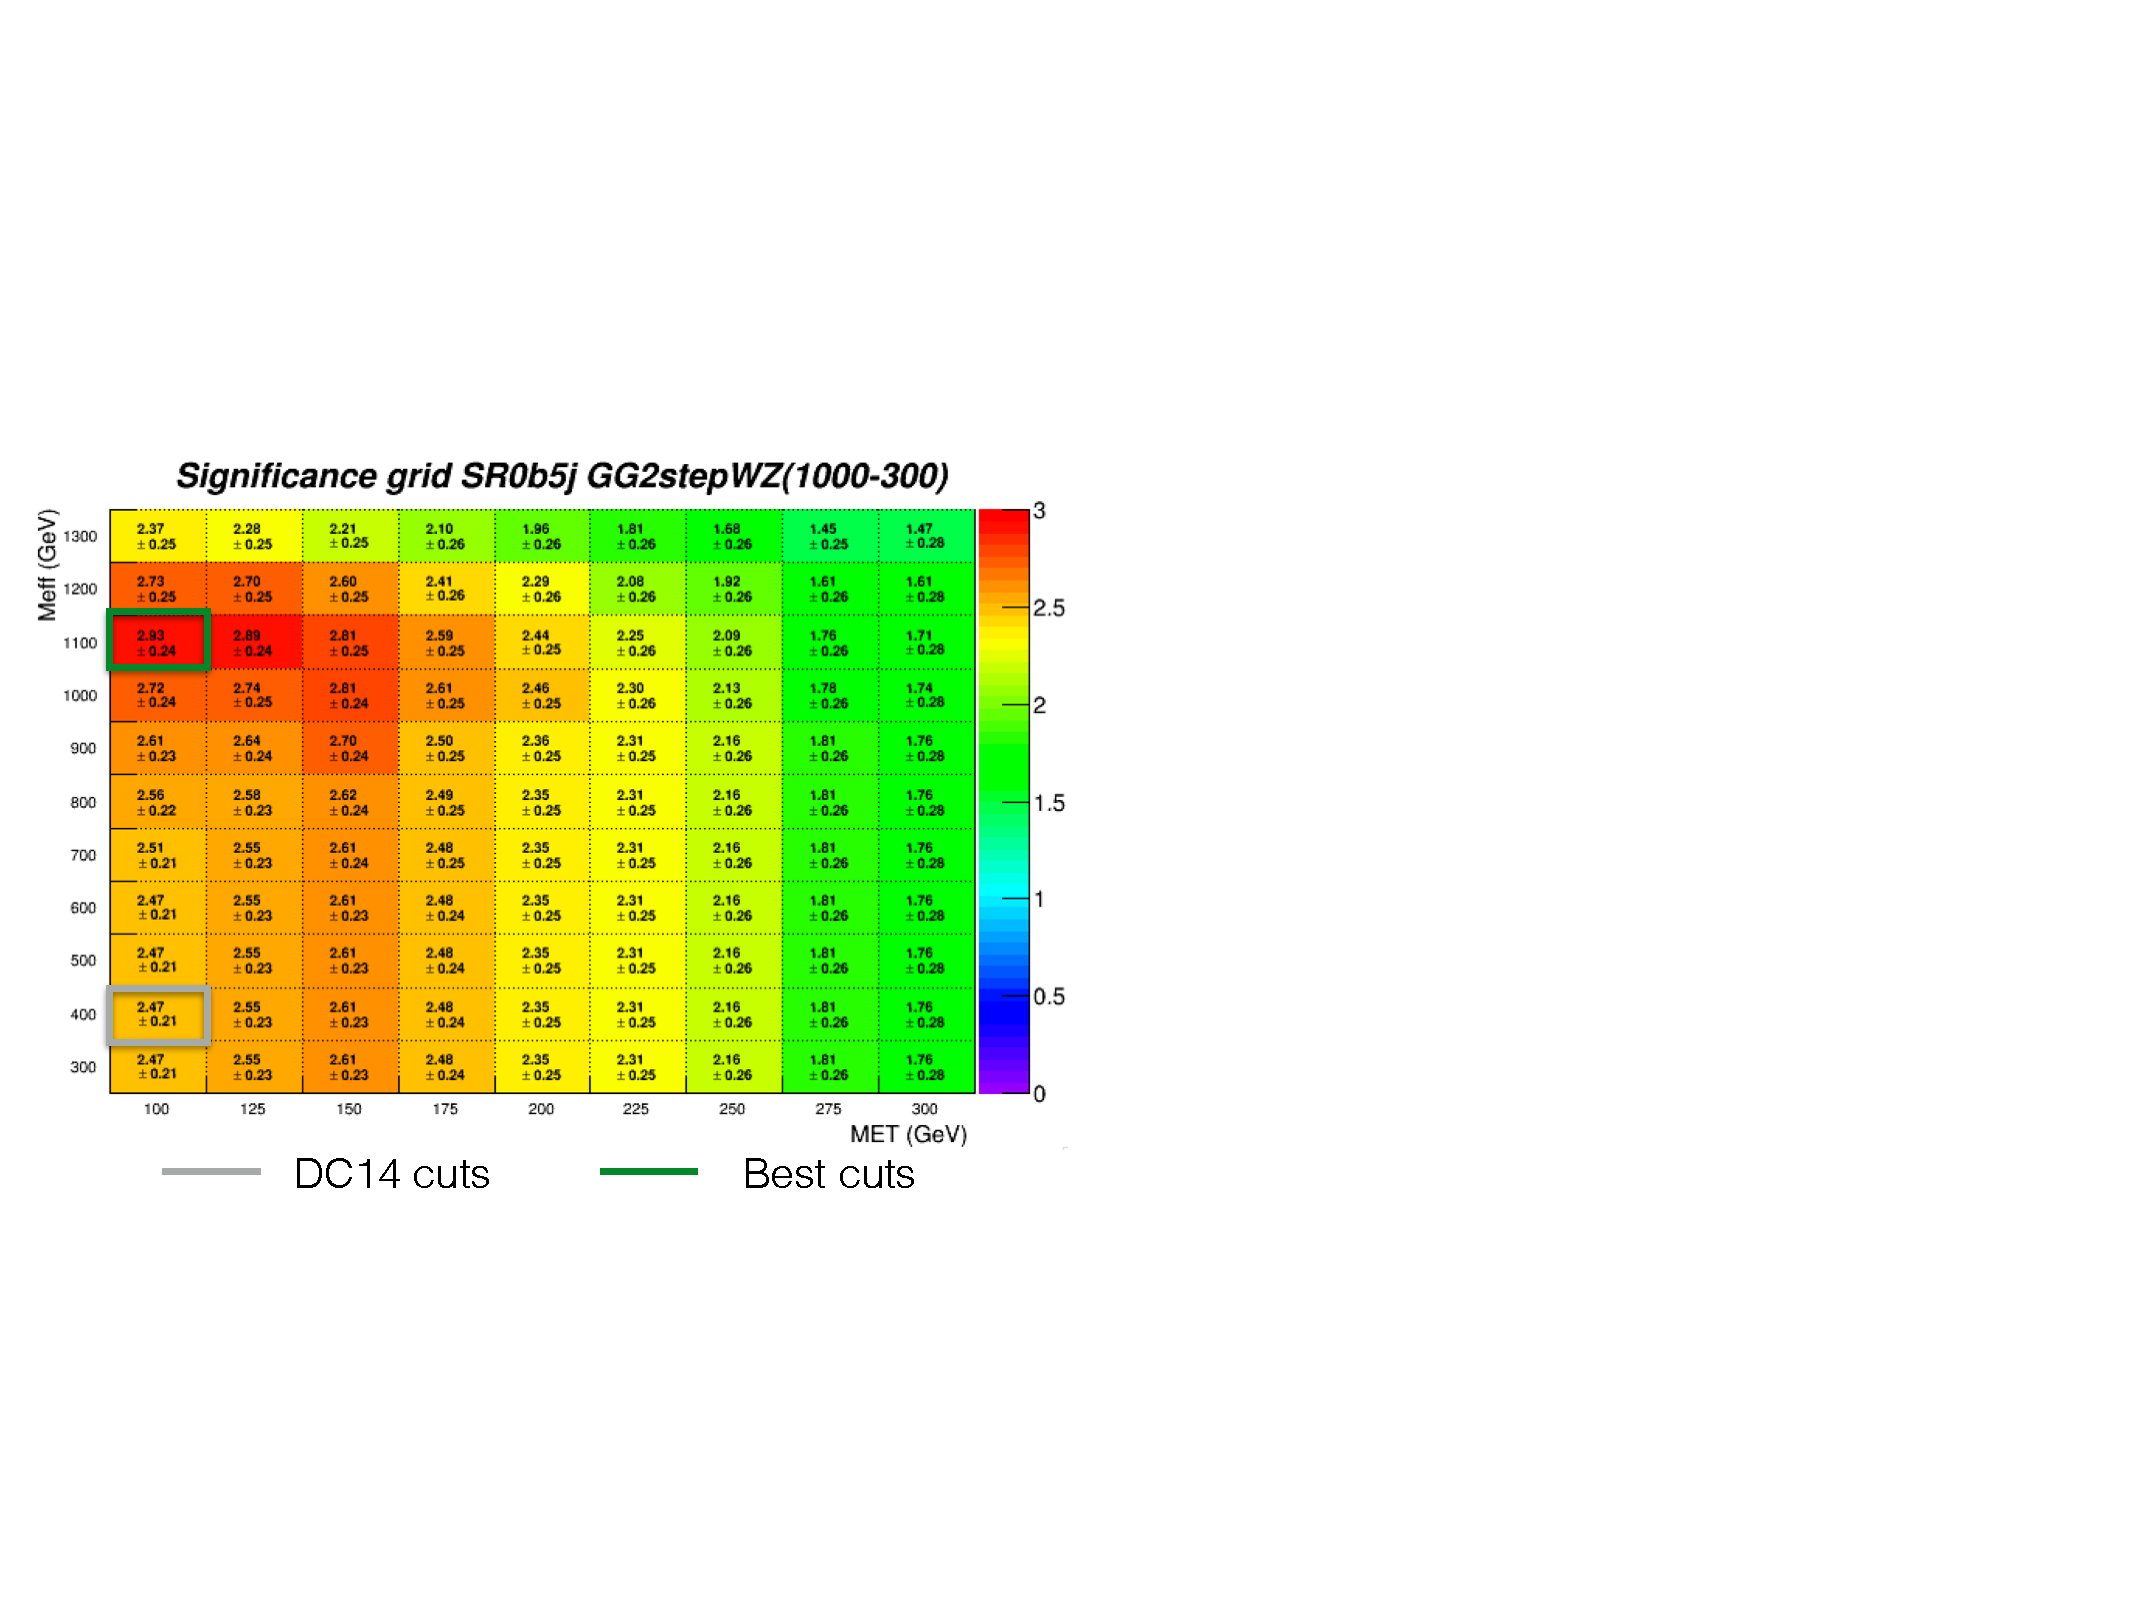
\includegraphics[width=0.49\textwidth]{OPTIMIZATION/Scan1.pdf}
  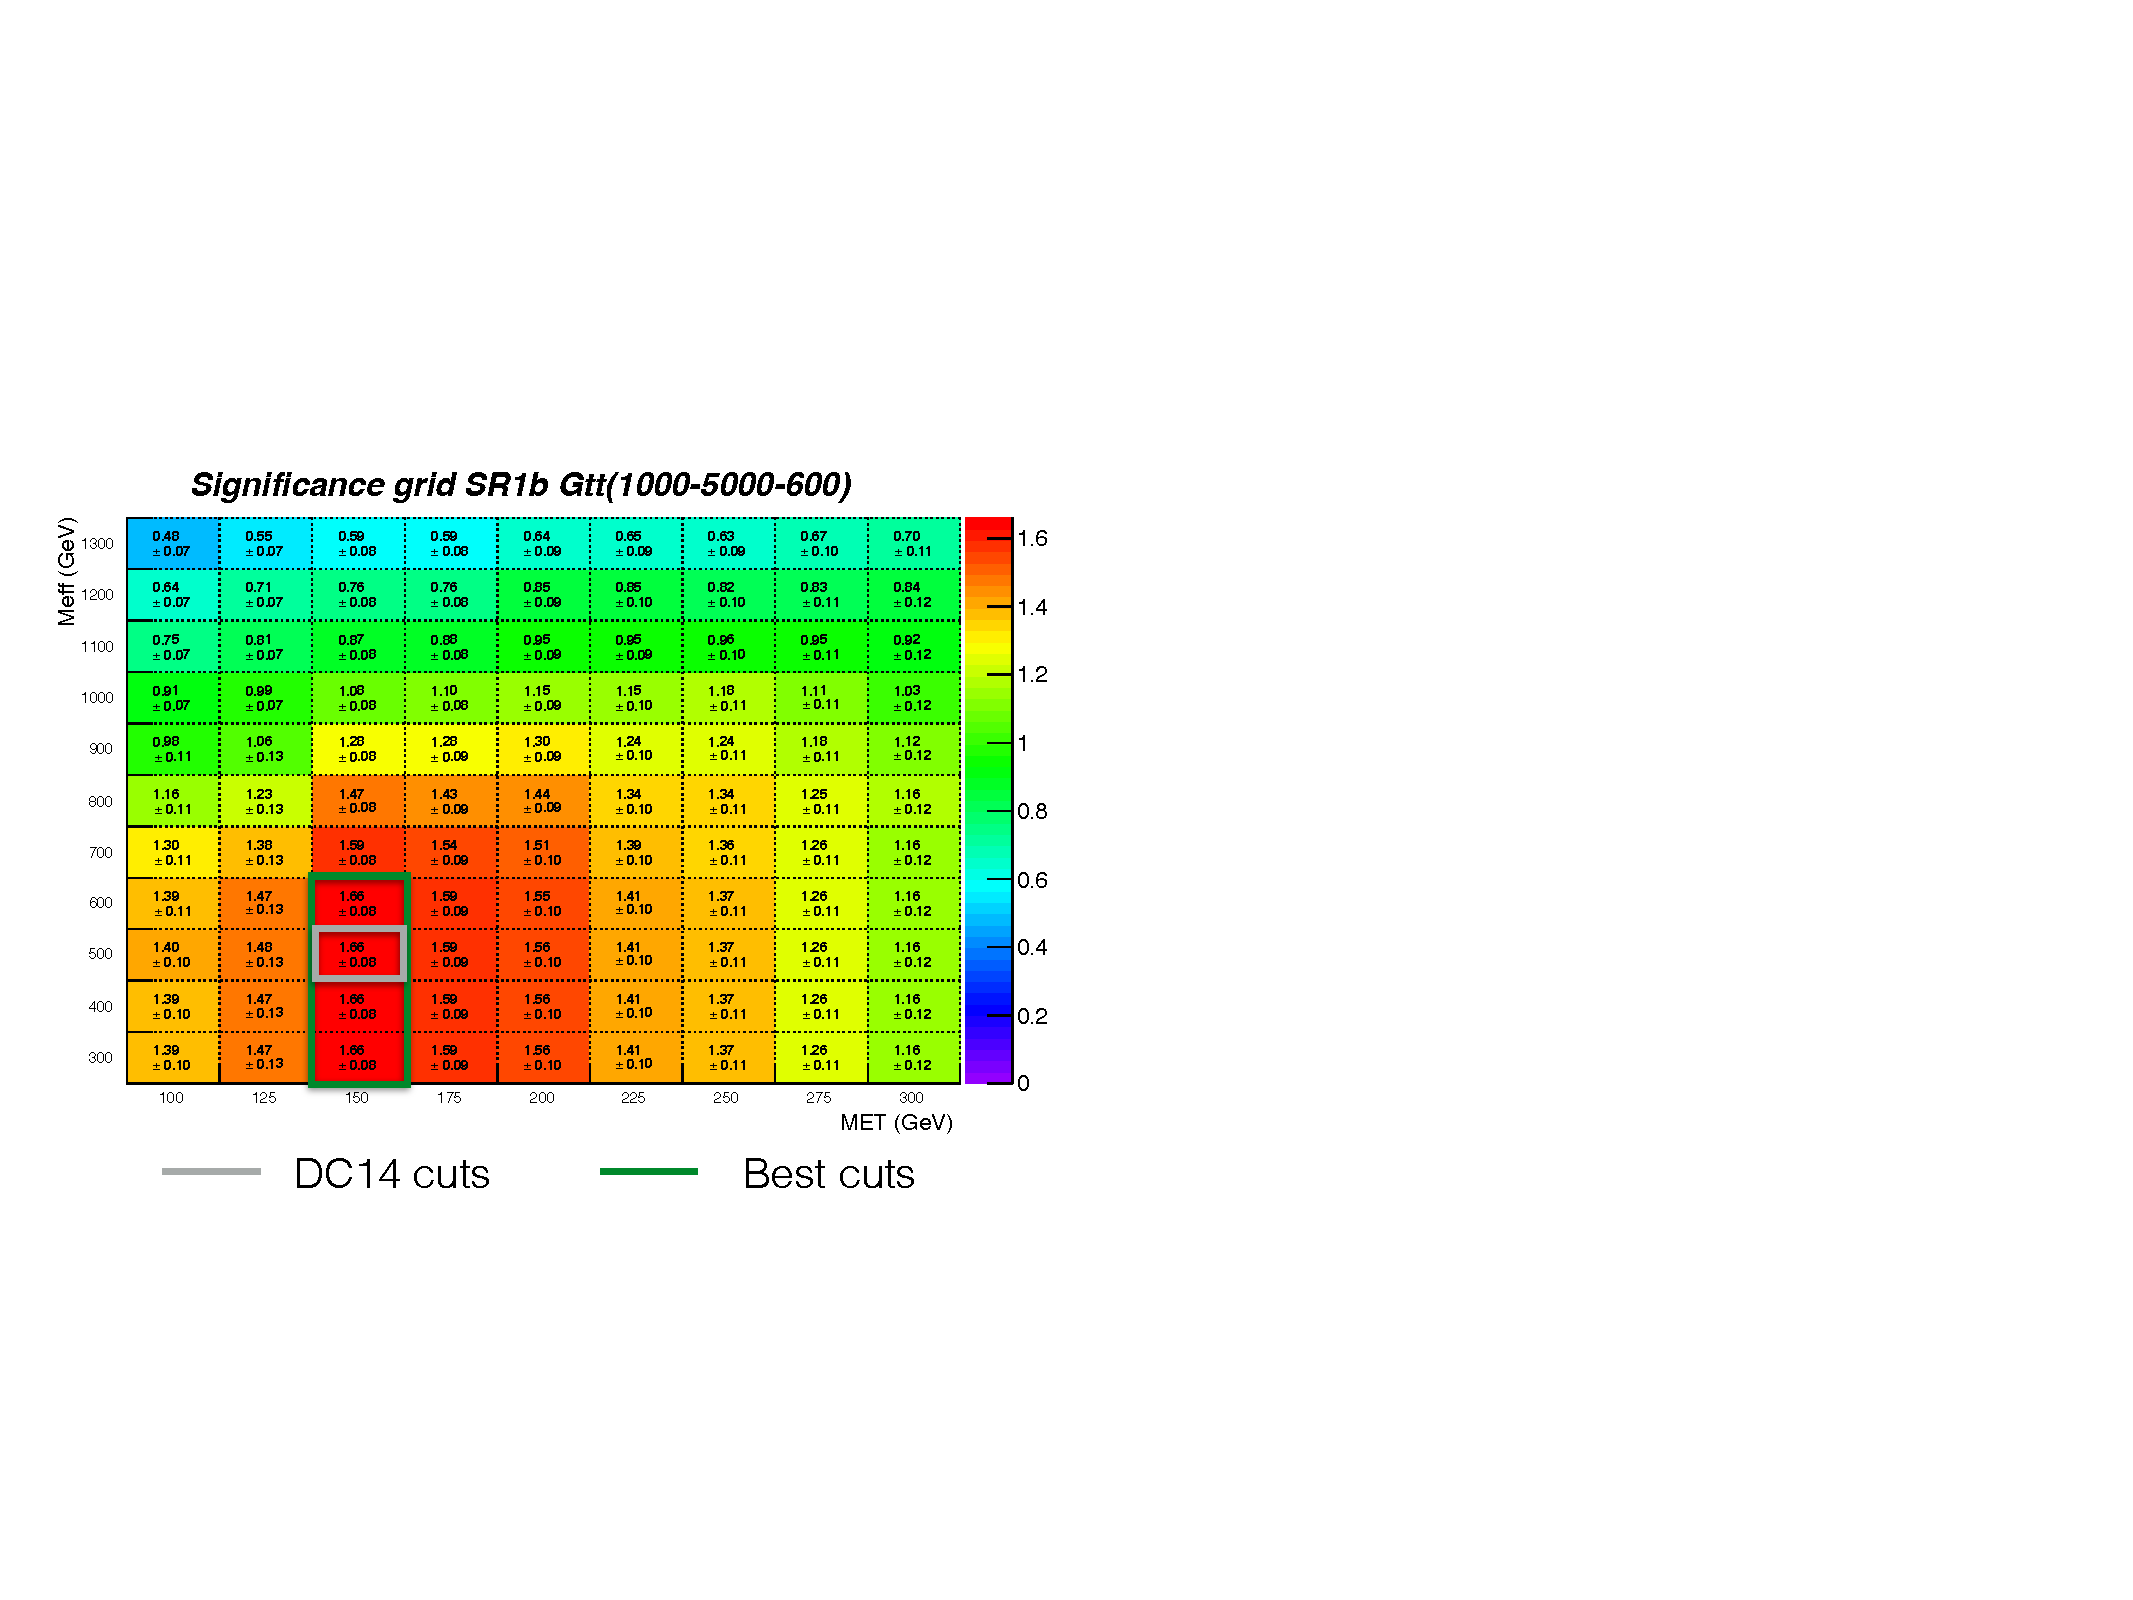
\includegraphics[width=0.49\textwidth]{OPTIMIZATION/Scan2.pdf}
  \caption{Example of (\met, \meff) scans for SR0b5j (left) and SR3b (right). The configurations with maximum significance are highlighted as well as the outcome of the DC14 optimization studies.}
\label{fig:OptimScan}


\end{figure}


%\begin{figure}[!htb]
%\centering
%  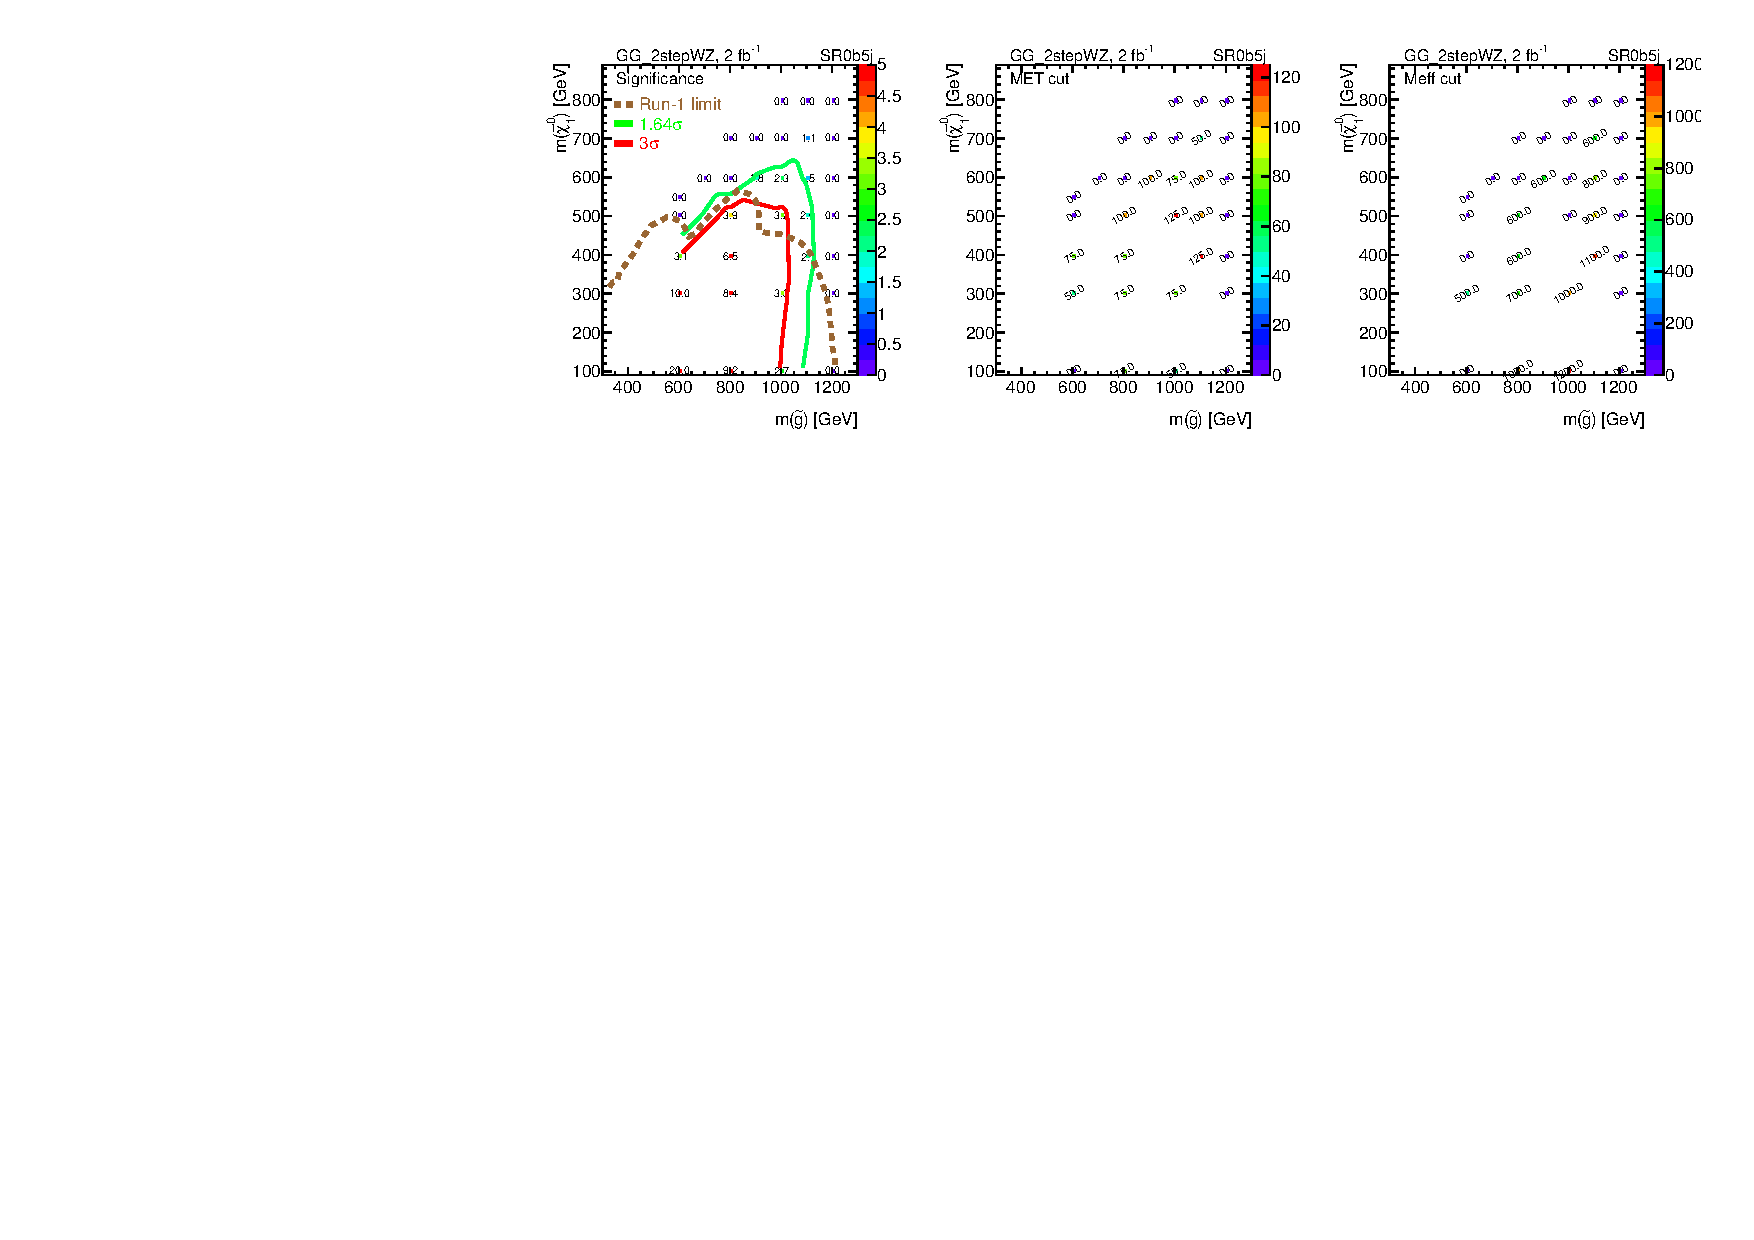
\includegraphics[width=\textwidth]{OPTIMIZATION/Optimiz_SR0b5j_2fb.pdf}
%  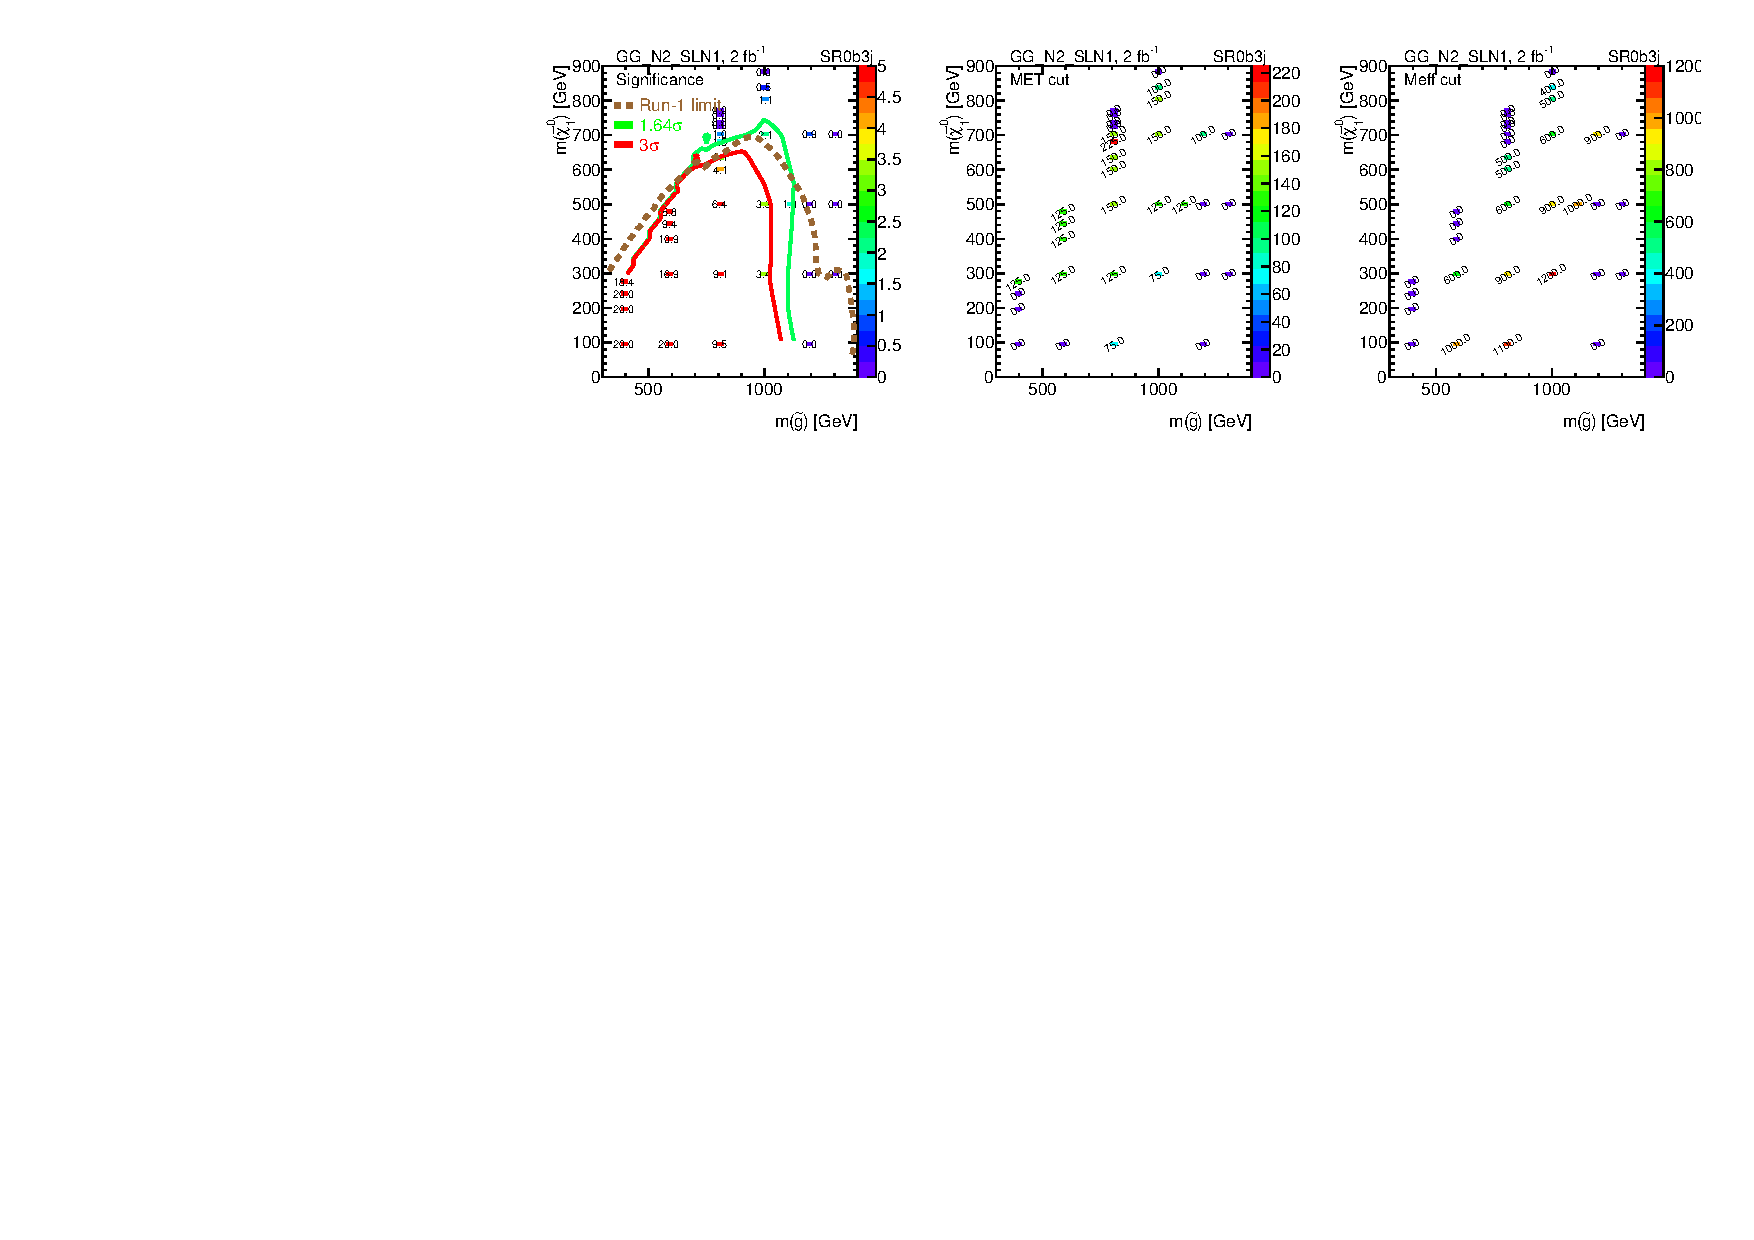
\includegraphics[width=\textwidth]{OPTIMIZATION/Optimiz_SR0b3j_2fb.pdf}
%\caption{Maximum discovery significance (left) for 2~\ifb\, as well as the $\met$ (center) and $\meff$ (right) cuts needed to maximize the significance for SR0b5j in the $\gluino\gluino$ 2-step grid (top) and SR0b3j in the $\gluino\gluino$ 1-step grid (bottom). The Run-1 limits in those models are shown with a brown line.}
%\label{fig:OptimSig2}
%\end{figure}


\subsection{Signal regions}
 
The definition of the exact SR was done as a good compromise across the signal grids shown in 
Figure~\ref{fig:OptimSig1} with a single ($\met$, $\meff$) configuration. 
Tables~\ref{tab:SRdef2}-\ref{tab:SRdef4} show the optimized signal region definitions for scenarios with 2, 3 and 4~\ifb\, respectively. 
The final SR to be used for the 2015 analysis was determined by the luminosity available at the end of the data-taking period: 
if less than 2.5~\ifb\ had been available for analysis after GRL, we would have used the SRs for the 2~\ifb\ scenario; 
if more than 3.5~\ifb\ had been available, we would have used the SRs for the 4~\ifb\ scenario. 
But with the 3.2~\ifb\ eventually collected, we used the definitions corresponding to the intermediate scenario of 3~\ifb.
Figures~\ref{fig:OptimSig2} and \ref{fig:OptimSig4} show the significance values obtained for those signal regions in the SUSY models considered, 
with the 1.64$\sigma$ discovery contours extending beyond the Run-1 exclusions, even achieving a 3$\sigma$ sensitivity in certain regions of the mass parameter space.
 
 
\begin{table}[htb!]
\caption{Signal regions definition for the 2~\ifb\ scenario (to be used for $L <2.5$~fb$^{-1}$). The two leading leptons are required to have \pt~$>$~20~\GeV.}
\hspace{0.5cm}
\label{tab:SRdef2}
\centering
\begin{tabular}{|c|c|c|c|c|c|}
\hline 
\hline
Signal region  &  $N_{\rm{lept}}$   & $N_{b\rm{-jets}}^{20}$    & $N_{\rm{jets}}^{50}$  & \met\ [GeV] & \meff\ [GeV]   \\
\hline\hline
SR3b     &   $\ge$2  &   $\ge$3  &  - & $>$100 & $>$600   \\
\hline
SR1b     &  $\ge$2  &    $\ge$1  &  $\ge$4 &  $>$125 & $>$500 \\
\hline
SR0b5j &  $\ge$2  &    $==$0 &  $\ge$5 &  $>$100 & $>$600 \\
\hline
SR0b3j &  $\ge$3  &    $==$0 &  $\ge$3 &  $>$150 & $>$500 \\
\hline\hline
\end{tabular}
\end{table}

\begin{table}[htb!]
\caption{Signal regions definition for the 3~\ifb\ scenario (to be used for $2.5 \leq L <3.5$~fb$^{-1}$), 
the one eventually used in this analysis. The two leading leptons are required to have \pt~$>$~20~\GeV.}
\hspace{0.5cm}
\label{tab:SRdef3}
\centering
\begin{tabular}{|c|c|c|c|c|c|}
\hline 
\hline
Signal region  &  $N_{\rm{lept}}$   & $N_{b\rm{-jets}}^{20}$    & $N_{\rm{jets}}^{50}$  & \met\ [GeV] & \meff\ [GeV]   \\
\hline\hline
SR3b     &   $\ge$2  &   $\ge$3  &  - & $>$125 & $>$650   \\
\hline
SR1b     &  $\ge$2  &    $\ge$1  &  $\ge$4 &  $>$150 & $>$550 \\
\hline
SR0b5j &  $\ge$2  &    $==$0 &  $\ge$5 &  $>$125 & $>$650 \\
\hline
SR0b3j &  $\ge$3  &    $==$0 &  $\ge$3 &  $>$200 & $>$550 \\
\hline\hline
\end{tabular}
\end{table}

\begin{table}[htb!]
\caption{Signal regions definition for the 4~\ifb\ scenario (to be used for $L \geq 3.5$~fb$^{-1}$). The two leading leptons are required to have \pt~$>$~20~\GeV.}
\hspace{0.5cm}
\label{tab:SRdef4}
\centering
\begin{tabular}{|c|c|c|c|c|c|}
\hline 
\hline
Signal region  &  $N_{\rm{lept}}$   & $N_{b\rm{-jets}}^{20}$    & $N_{\rm{jets}}^{50}$  & \met\ [GeV] & \meff\ [GeV]   \\
\hline\hline
SR3b     &   $\ge$2  &   $\ge$3  &  - & $>$125 & $>$700   \\
\hline
SR1b     &  $\ge$2  &    $\ge$1  &  $\ge$4 &  $>$150 & $>$600 \\
\hline
SR0b5j &  $\ge$2  &    $==$0 &  $\ge$5 &  $>$125 & $>$700 \\
\hline
SR0b3j &  $\ge$3  &    $==$0 &  $\ge$3 &  $>$200 & $>$600 \\
\hline\hline
\end{tabular}
\end{table}

\begin{figure}[!htb]
\centering
  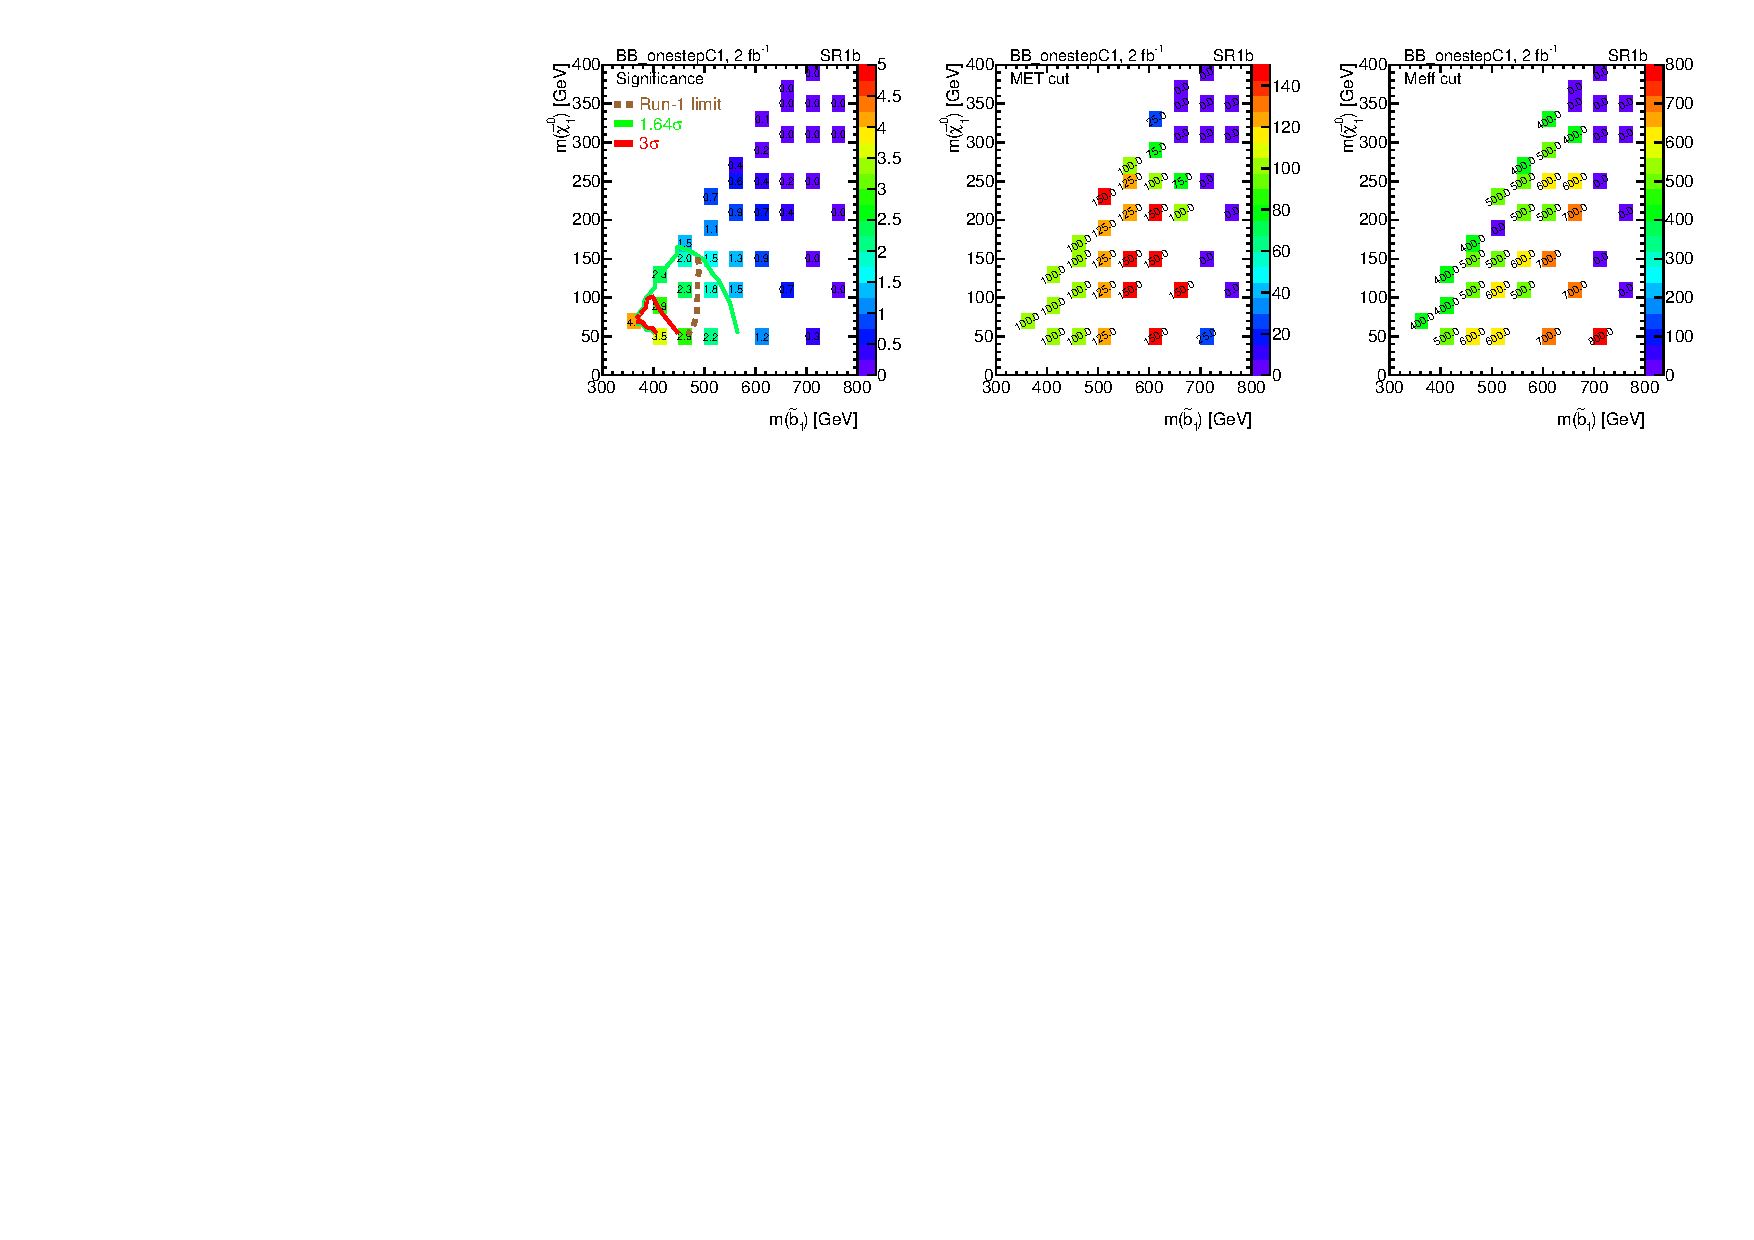
\includegraphics[width=0.9\textwidth]{OPTIMIZATION/Optimiz_SR1b_2fb.pdf}
  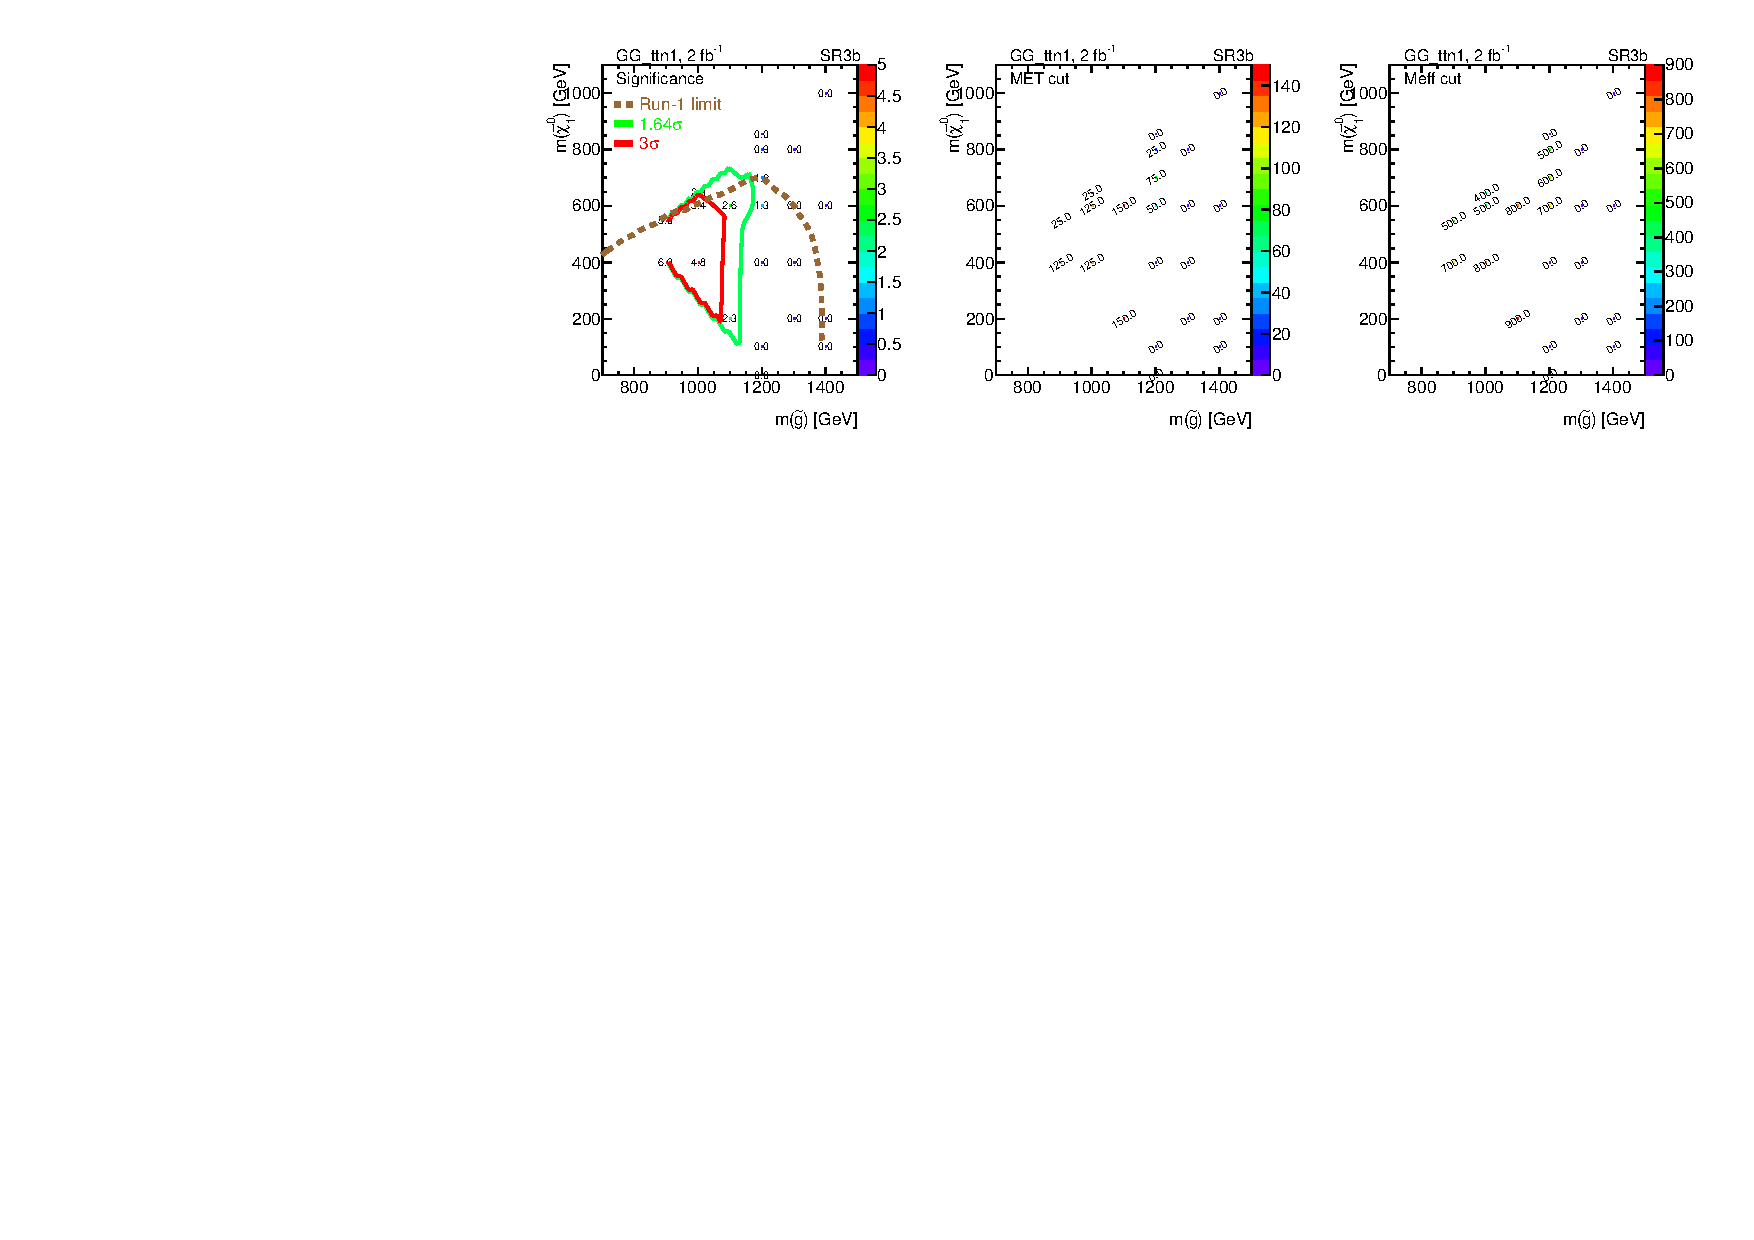
\includegraphics[width=0.9\textwidth]{OPTIMIZATION/Optimiz_SR3b_2fb.pdf}
  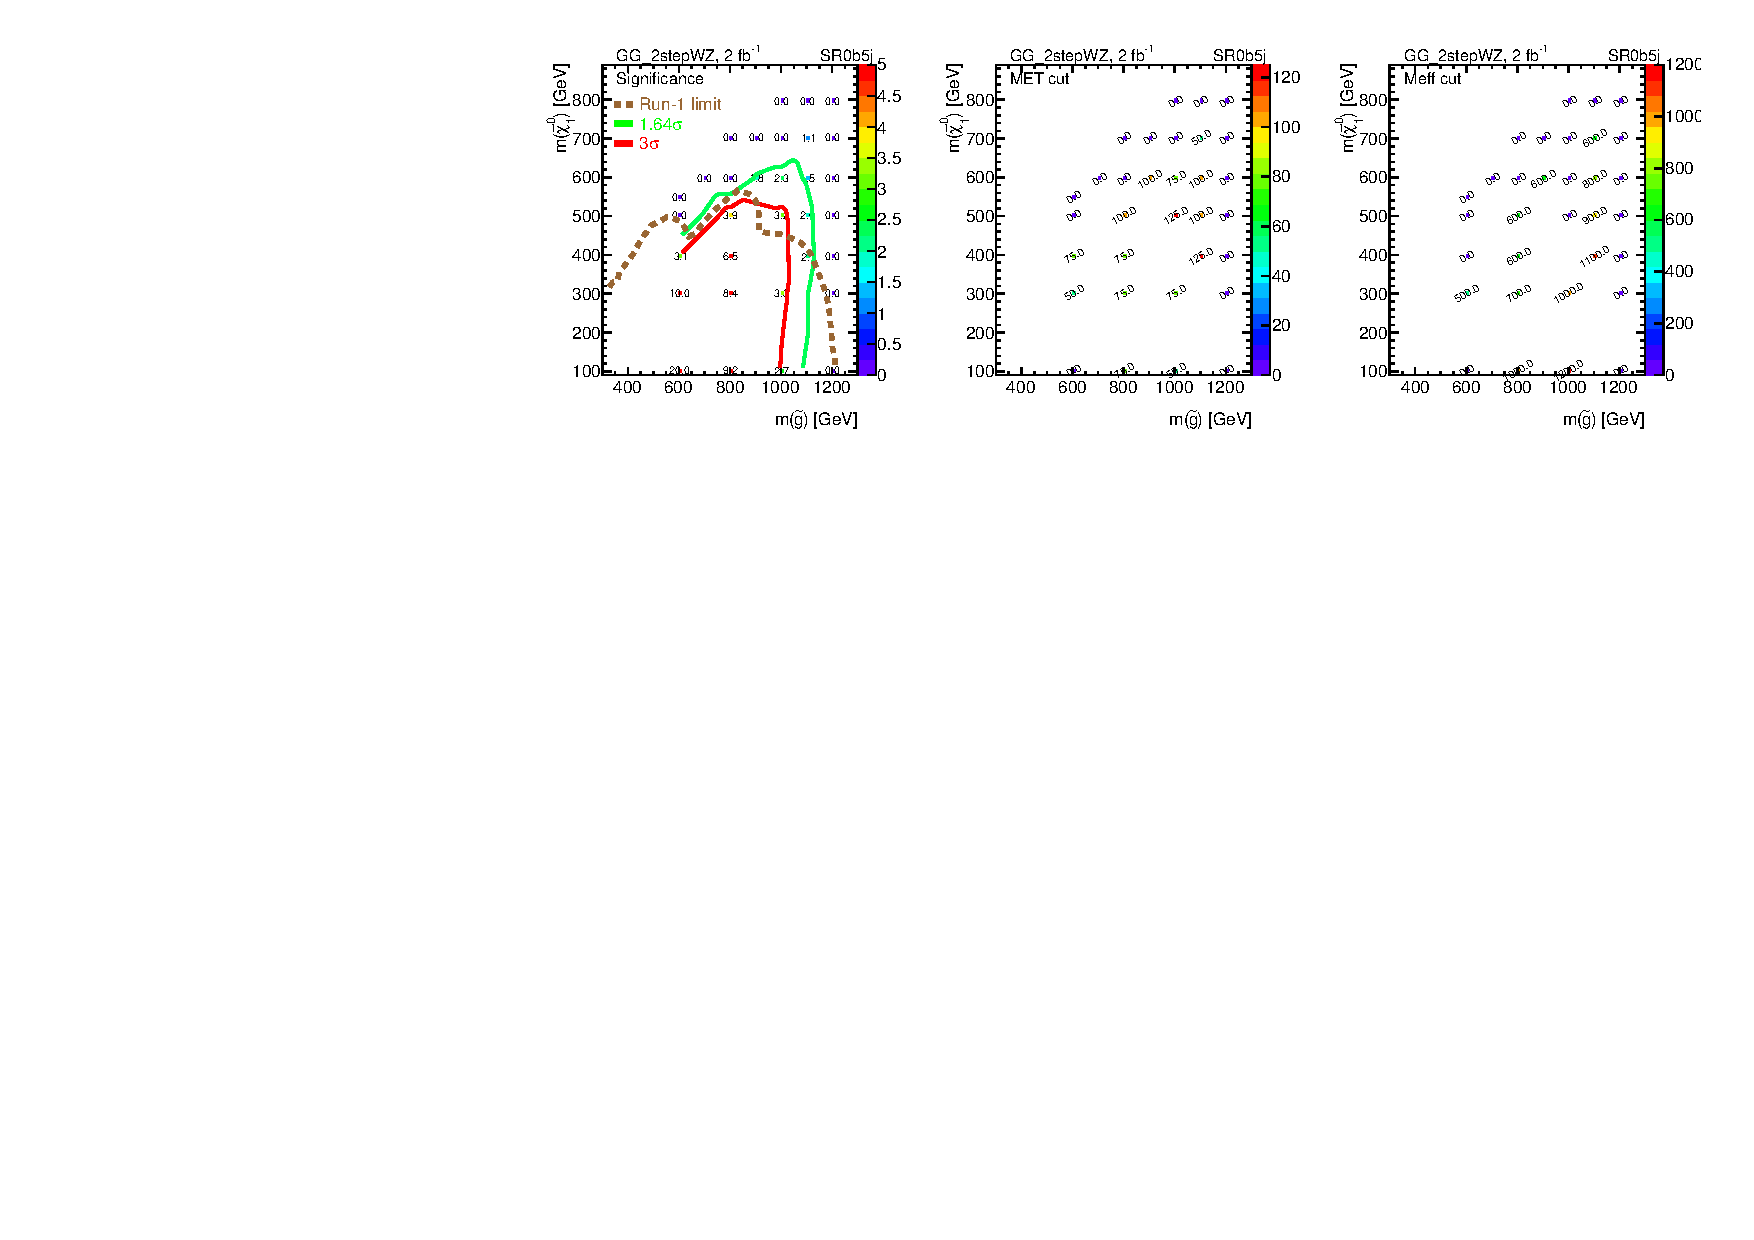
\includegraphics[width=0.9\textwidth]{OPTIMIZATION/Optimiz_SR0b5j_2fb.pdf}
  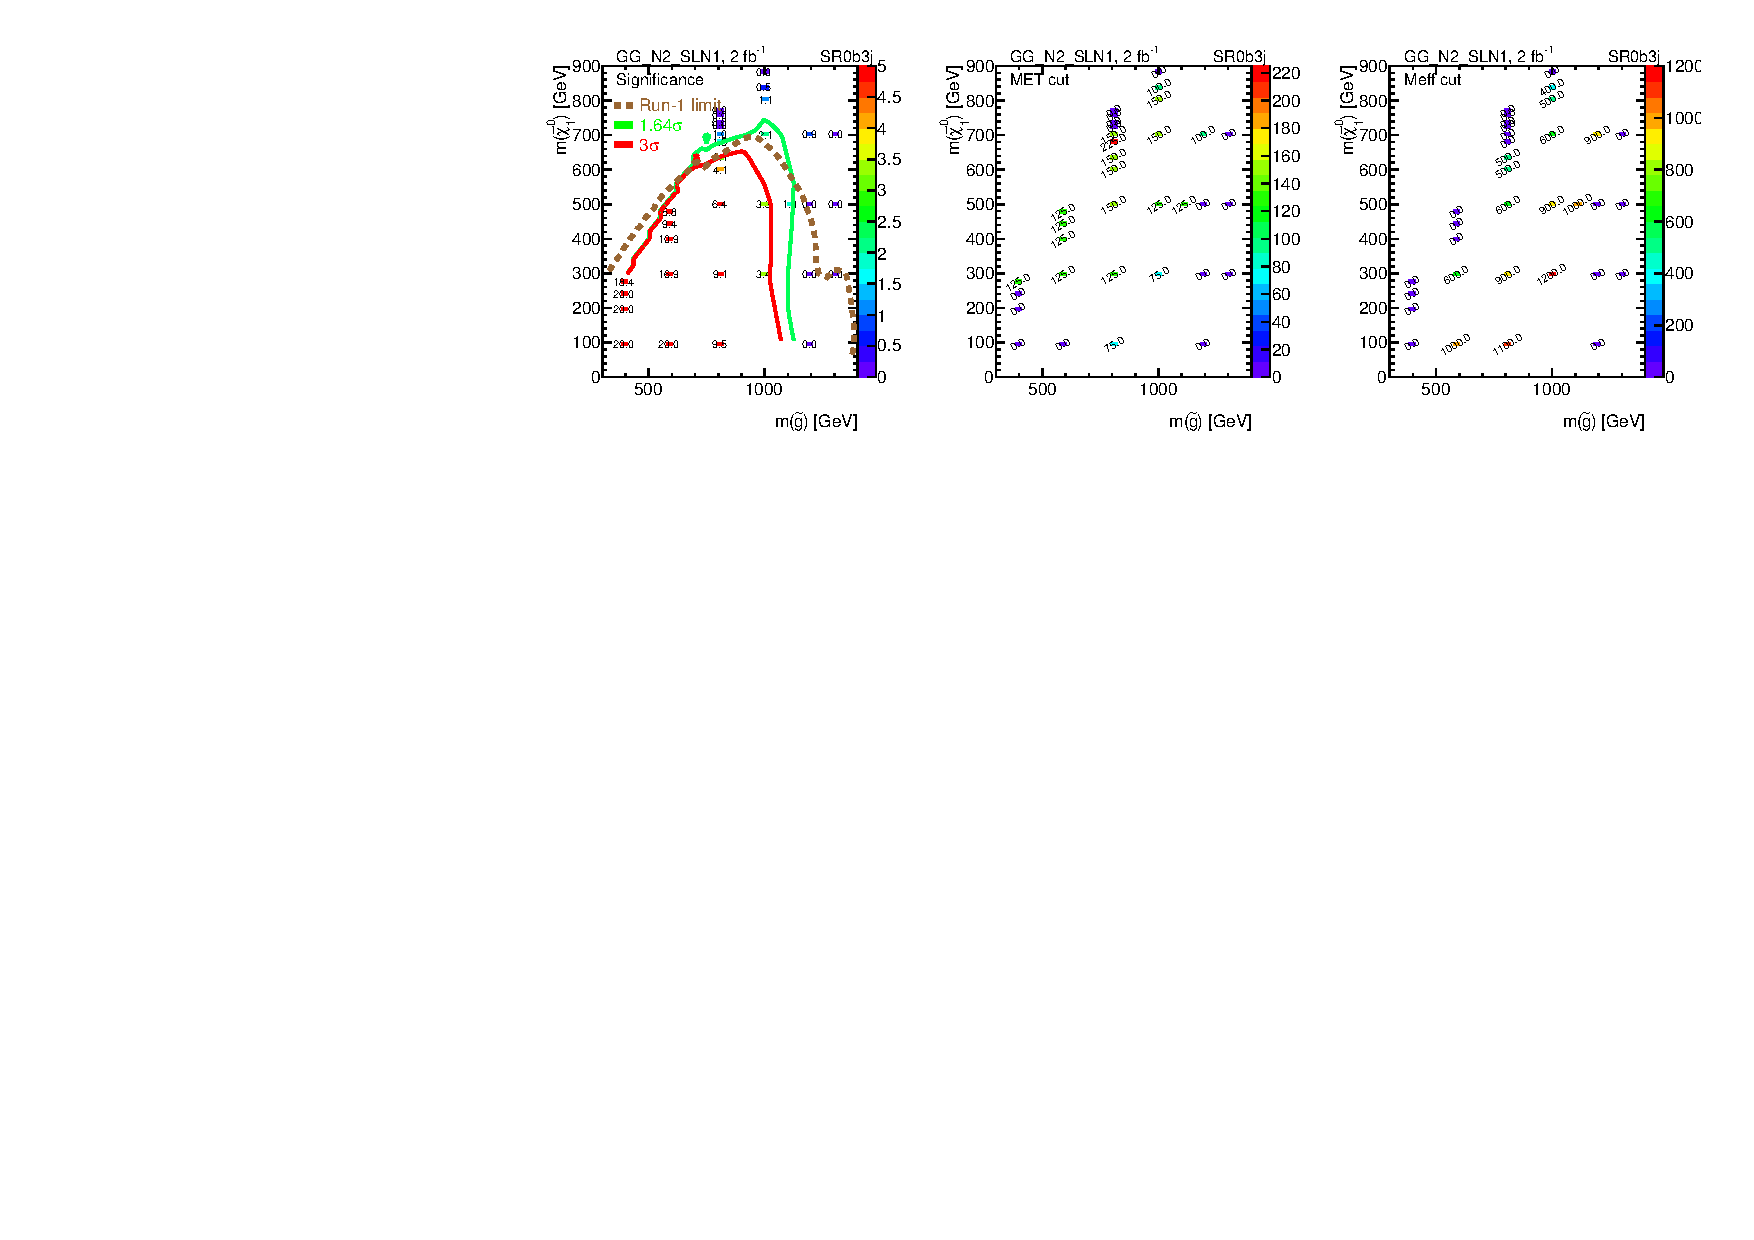
\includegraphics[width=0.9\textwidth]{OPTIMIZATION/Optimiz_SR0b3j_2fb.pdf}
  \caption{Maximum discovery significance (left) for 2~\ifb, as well as the $\met$ (center) and $\meff$ (right) cuts needed to maximize the significance for: (from top to bottom) SR1b in the $\sbot\sbot^*\to t\bar t\tilde\chi_1^+\tilde\chi_1^-$ grid, SR3b in the $\gluino\gluino\to t\bar tt\bar t\ninoone\ninoone$ grid, SR0b5j in the $\gluino\gluino$ with $\gluino\to q\bar{q}'WZ\ninoone$ grid and SR0b3j in the $\gluino\gluino$ with $\gluino\to q\bar{q}(\ell\ell/\ell\nu)\ninoone$ grid. The Run-1 limits in those models are shown with a brown line, and the 1.64$\sigma$ and 3$\sigma$ discovery contours from the proposed signal regions are shown in green and red, respectively.}
\label{fig:OptimSig1}
\end{figure}



\begin{figure}[!htb]
\centering
  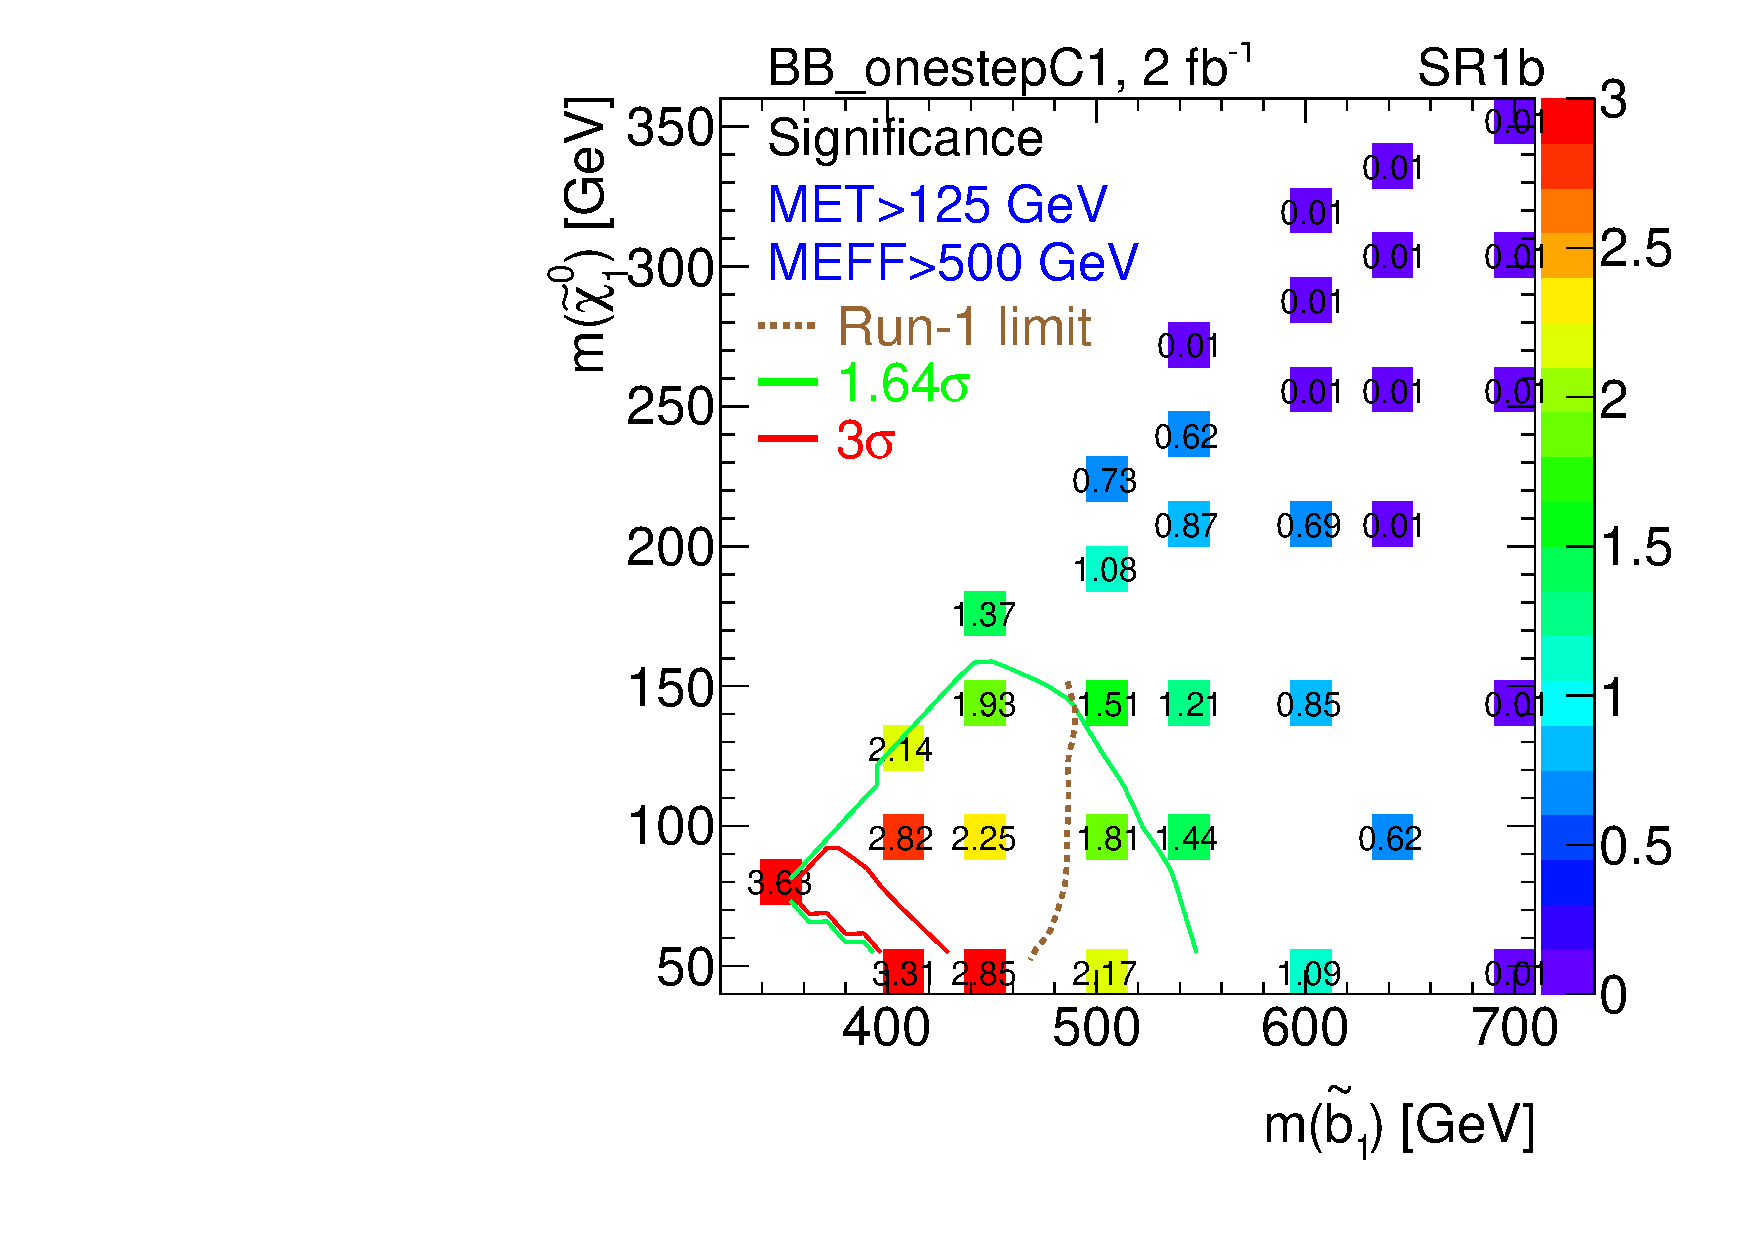
\includegraphics[width=0.4\textwidth]{OPTIMIZATION/Optimiz_SR1b_2fb_125_500.pdf}
  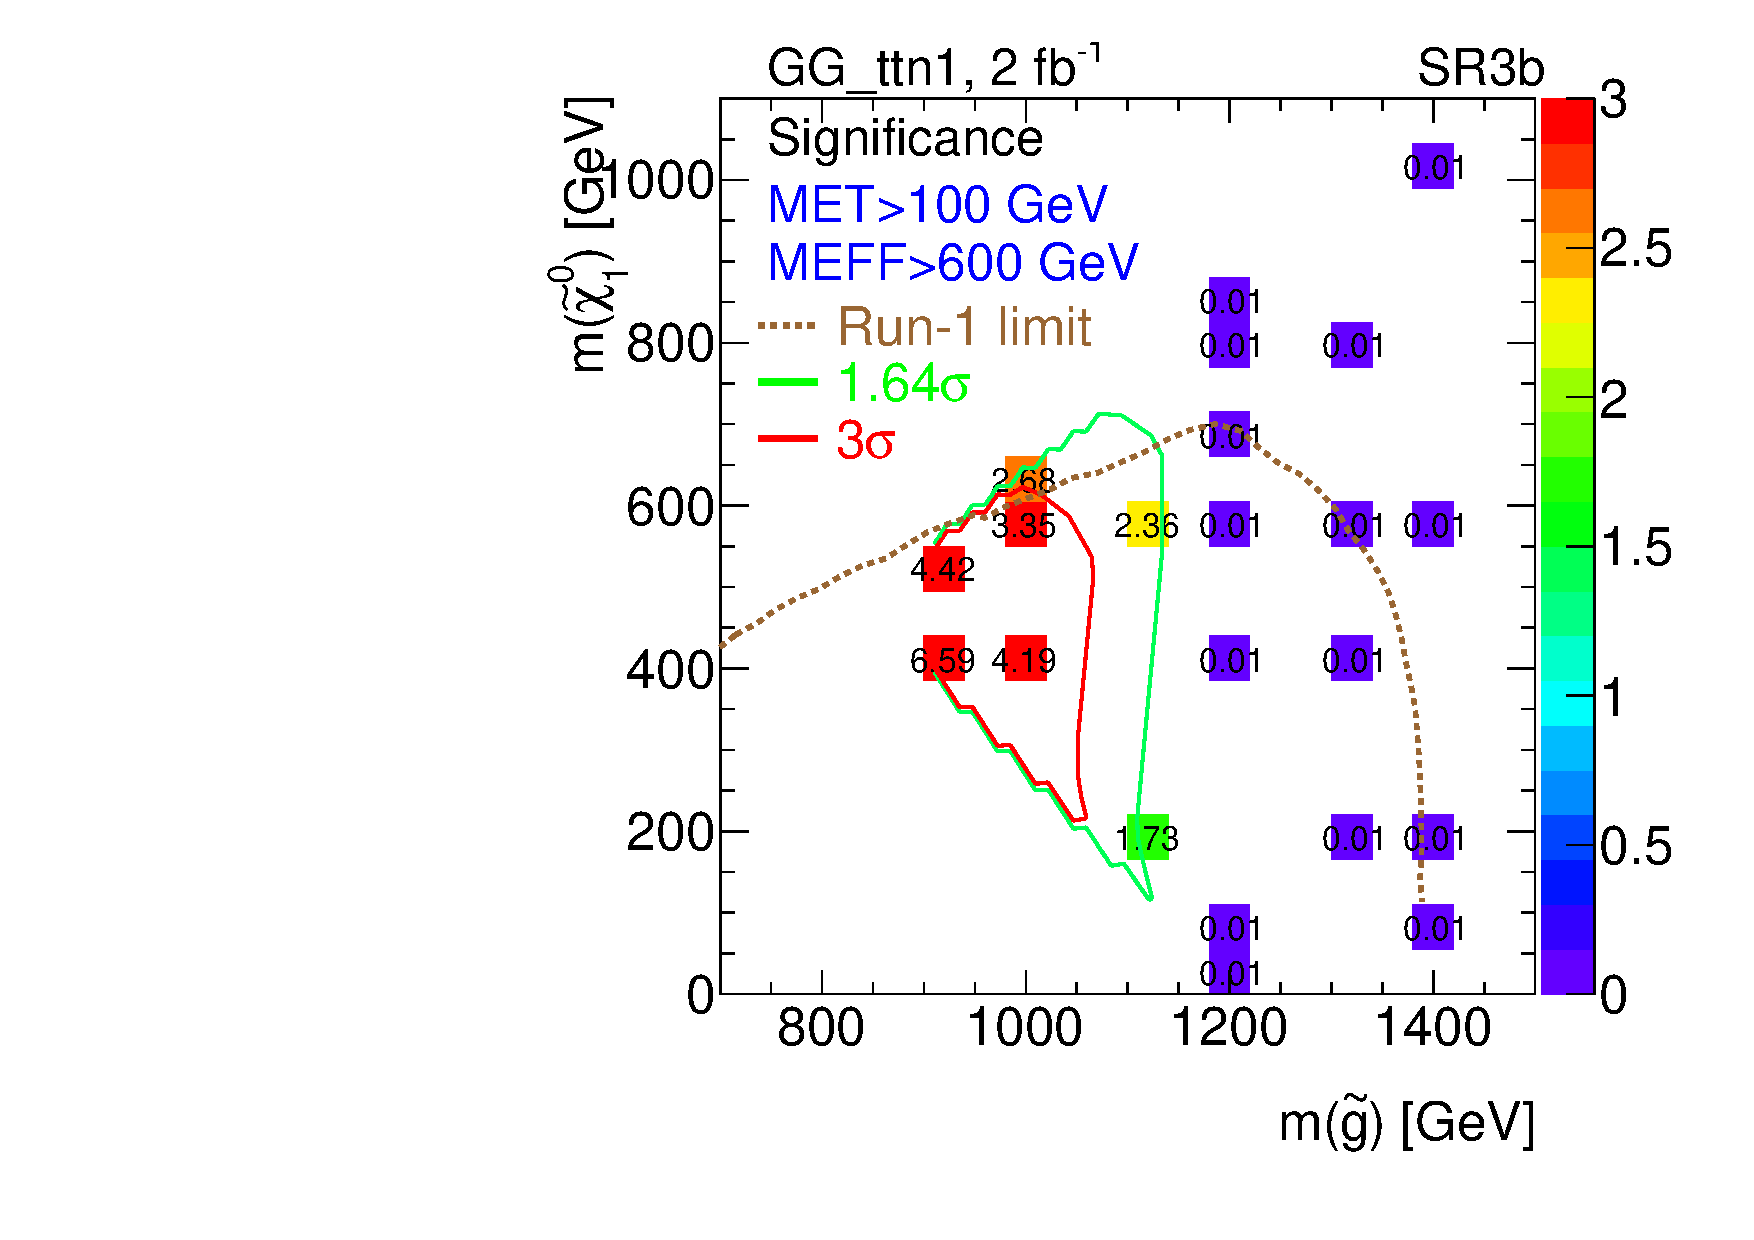
\includegraphics[width=0.4\textwidth]{OPTIMIZATION/Optimiz_SR3b_2fb_100_600.pdf}\\
  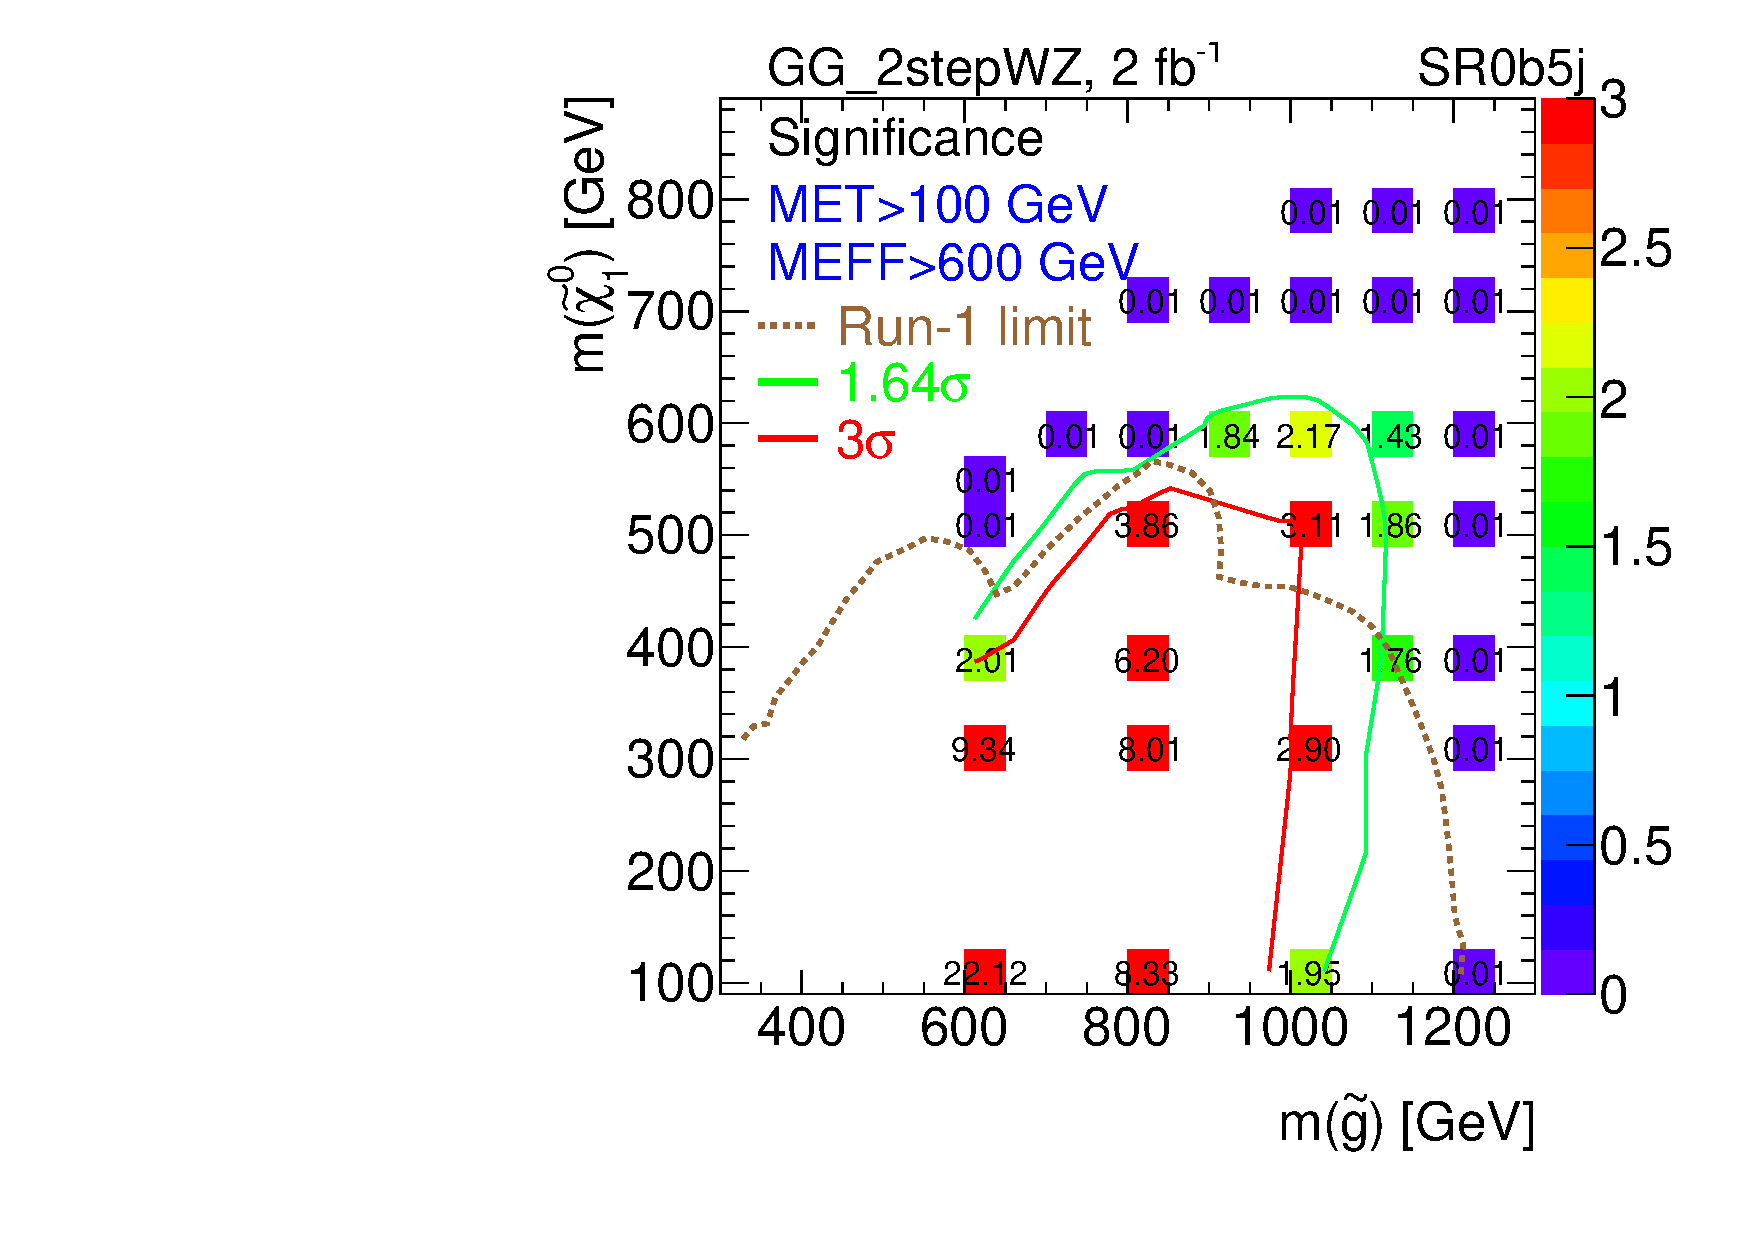
\includegraphics[width=0.4\textwidth]{OPTIMIZATION/Optimiz_SR0b5j_2fb_100_600.pdf}
  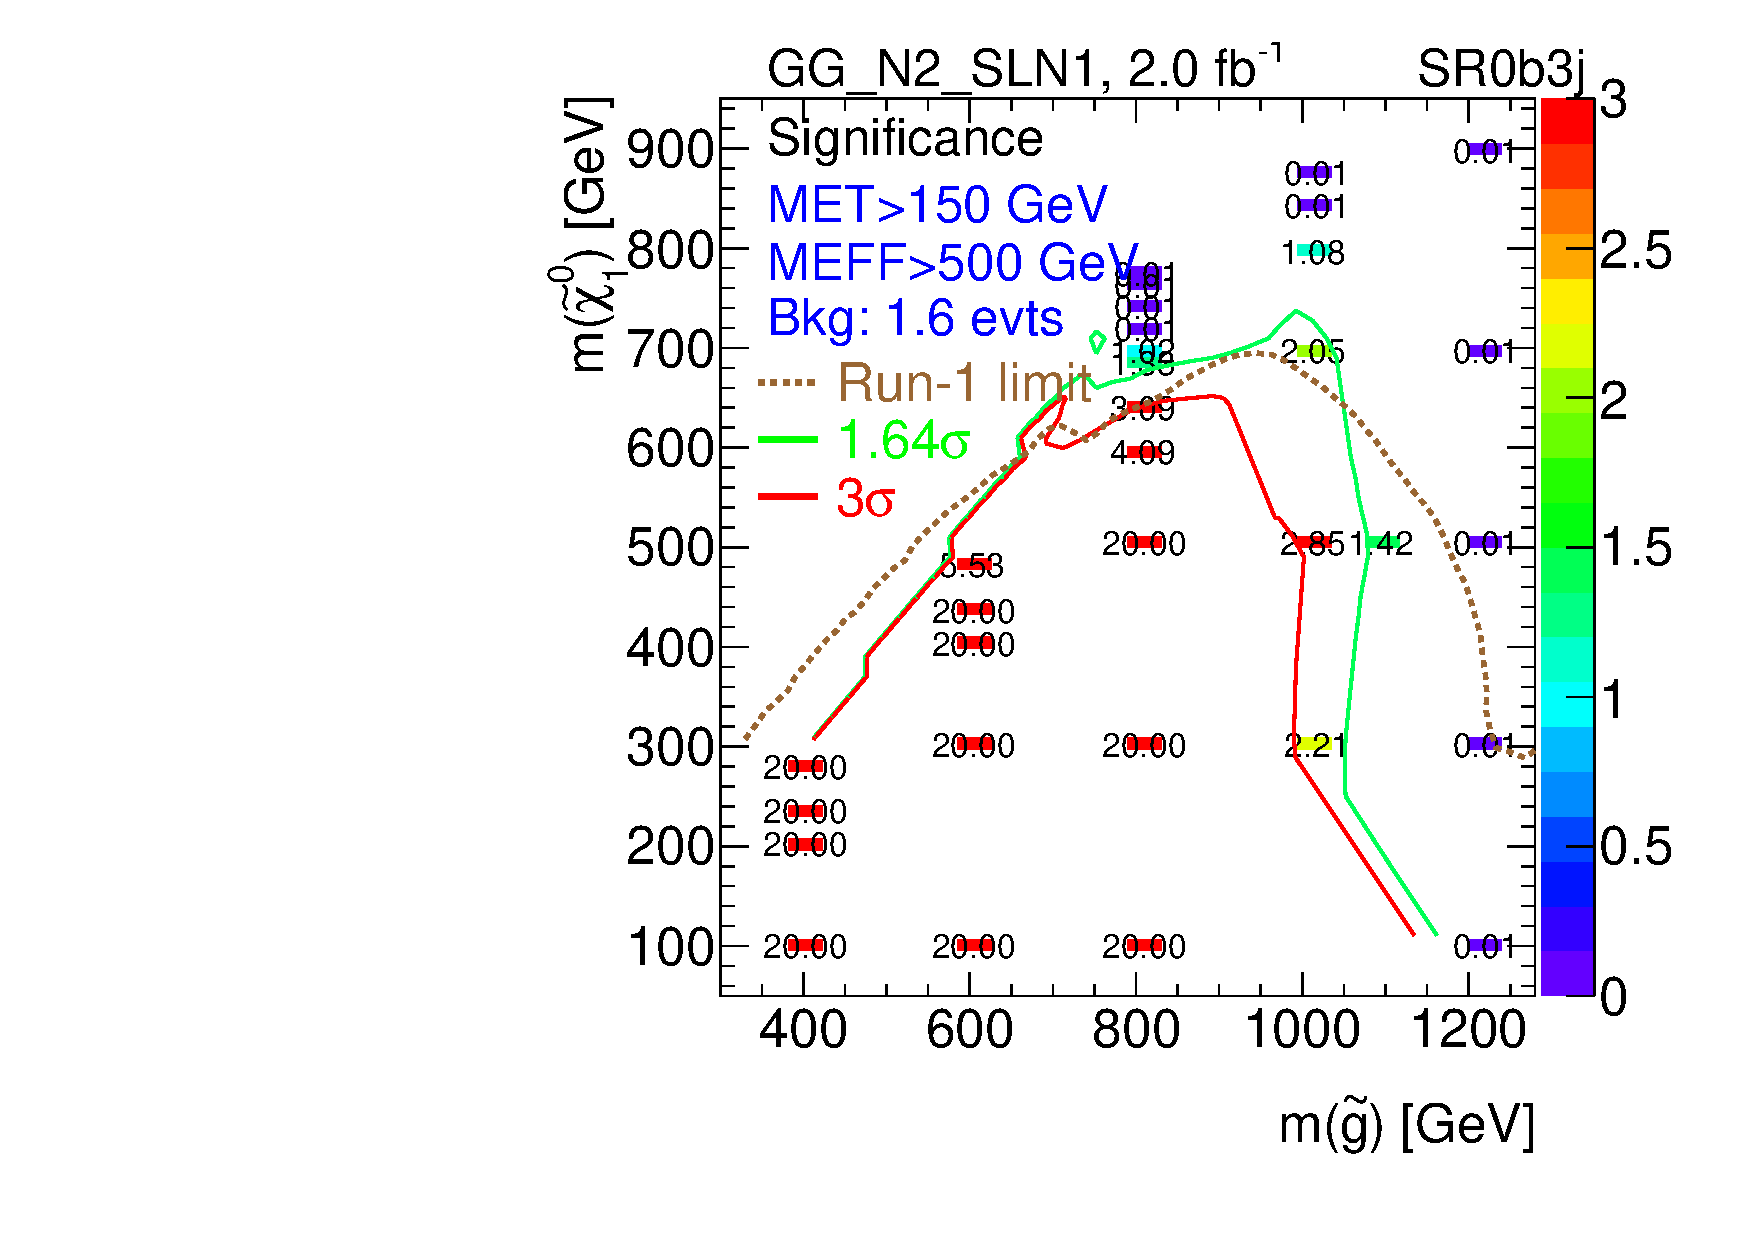
\includegraphics[width=0.4\textwidth]{OPTIMIZATION/Optimiz_SR0b3j_2fb_150_500.pdf}
  \caption{Discovery significance for the SRs defined in Table~\ref{tab:SRdef2} (2~\ifb) for SR1b in the $\sbot\sbot^*\to t\bar t\tilde\chi_1^+\tilde\chi_1^-$ grid (top left), SR3b in the $\gluino\gluino\to t\bar tt\bar t\ninoone\ninoone$ grid (top right), SR0b5j in the $\gluino\gluino$ with $\gluino\to q\bar{q}'WZ\ninoone$ grid (bottom left) and SR0b3j in the $\gluino\gluino$ with $\gluino\to q\bar{q}(\ell\ell/\ell\nu)\ninoone$ grid (bottom right). The Run-1 limits in those models are shown with a brown line, and the 1.64$\sigma$ and 3$\sigma$ discovery contours from the proposed signal regions are shown in green and red, respectively.}
\label{fig:OptimSig2}
\end{figure}


\begin{figure}[!htb]
\centering
  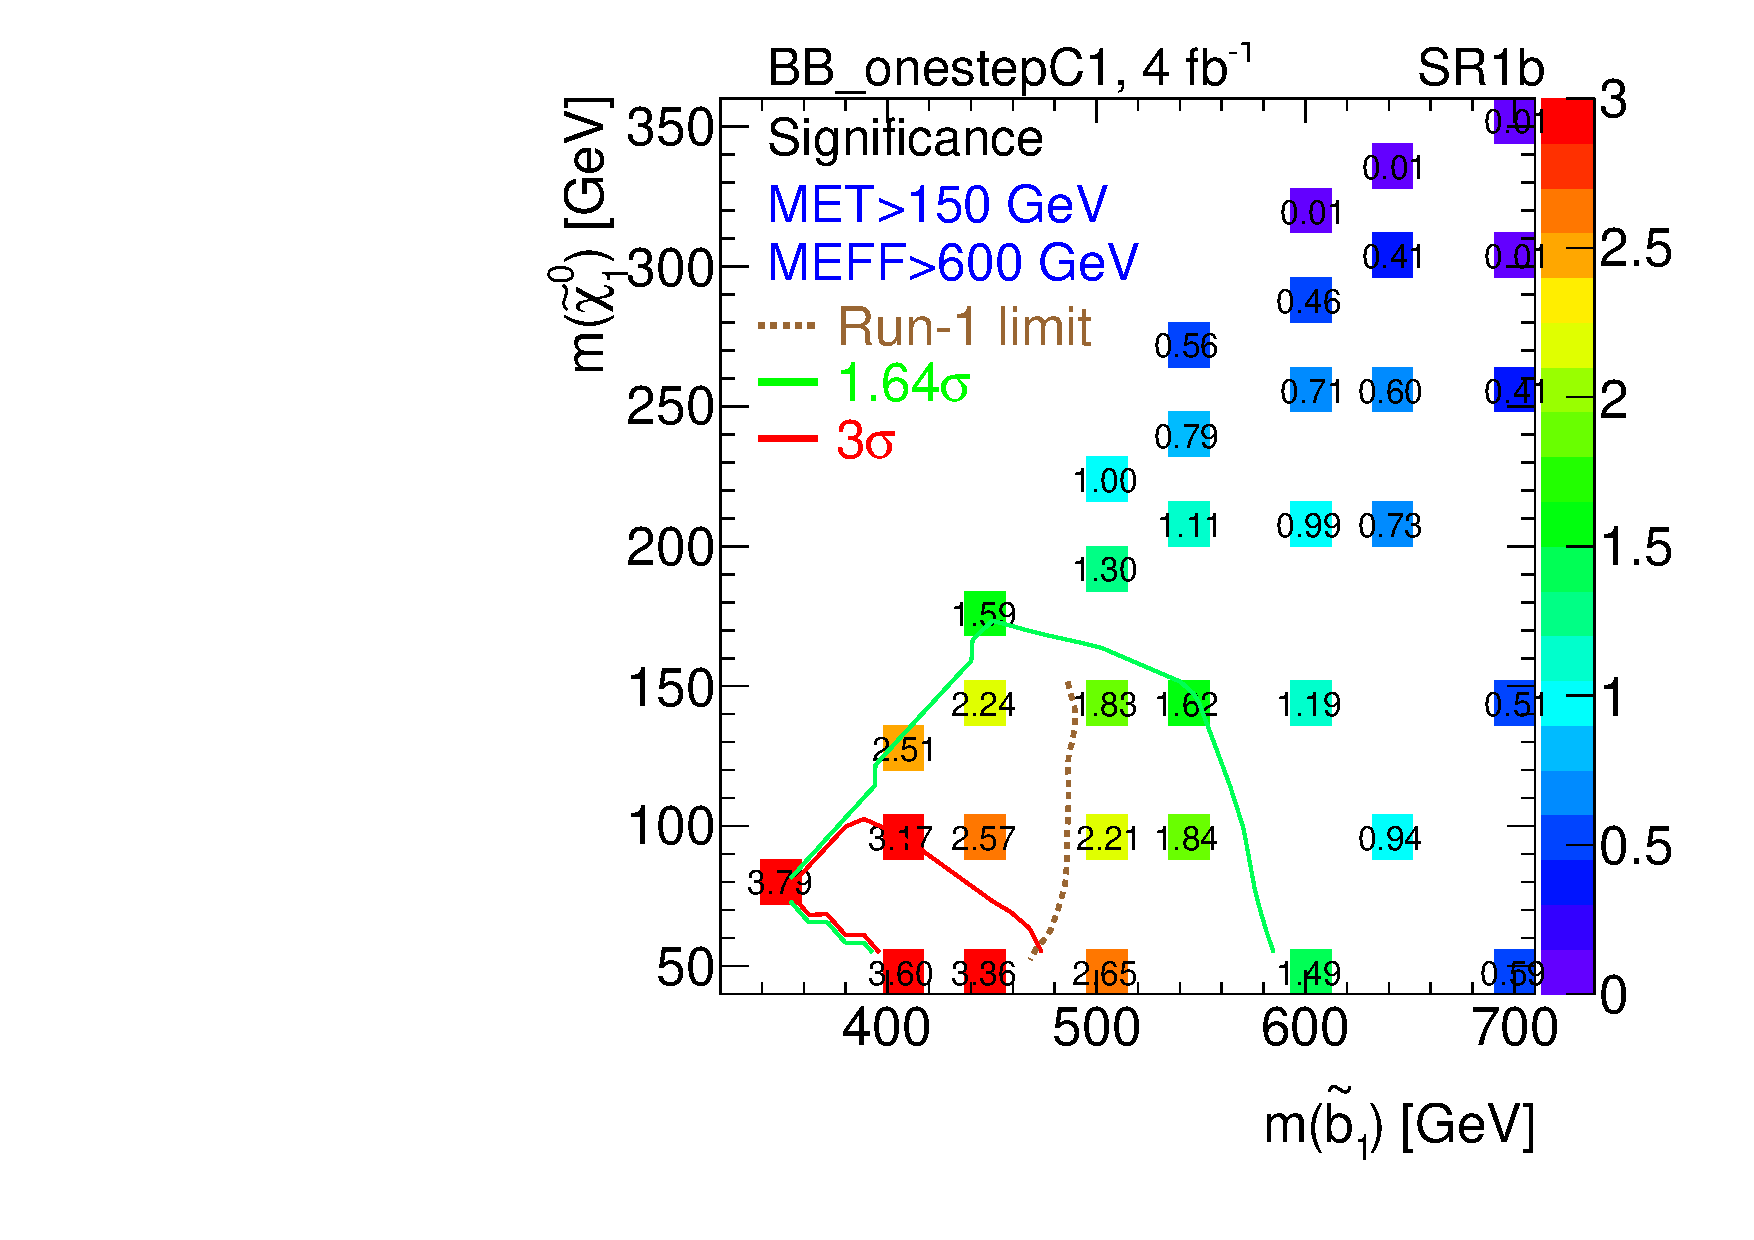
\includegraphics[width=0.4\textwidth]{OPTIMIZATION/Optimiz_SR1b_4fb_150_600.pdf}
  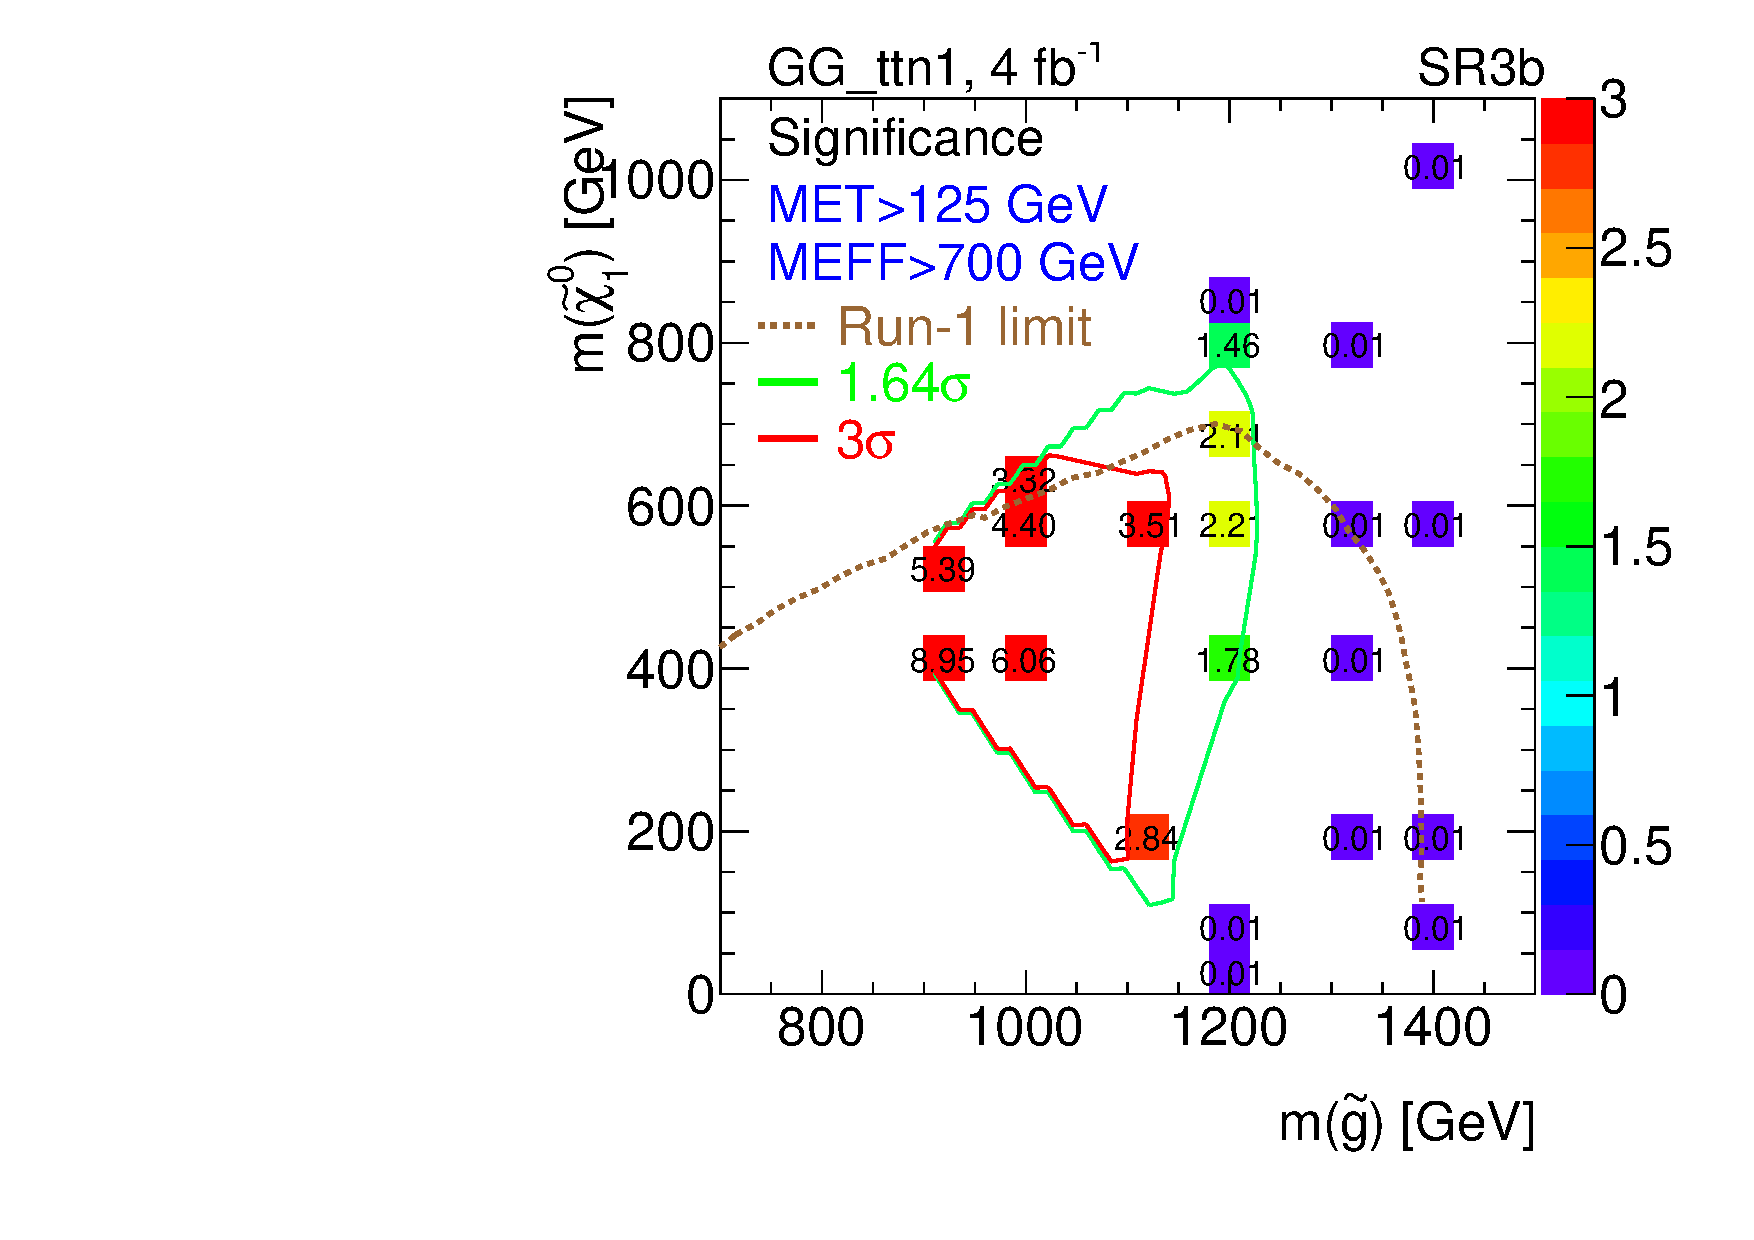
\includegraphics[width=0.4\textwidth]{OPTIMIZATION/Optimiz_SR3b_4fb_125_700.pdf}\\
  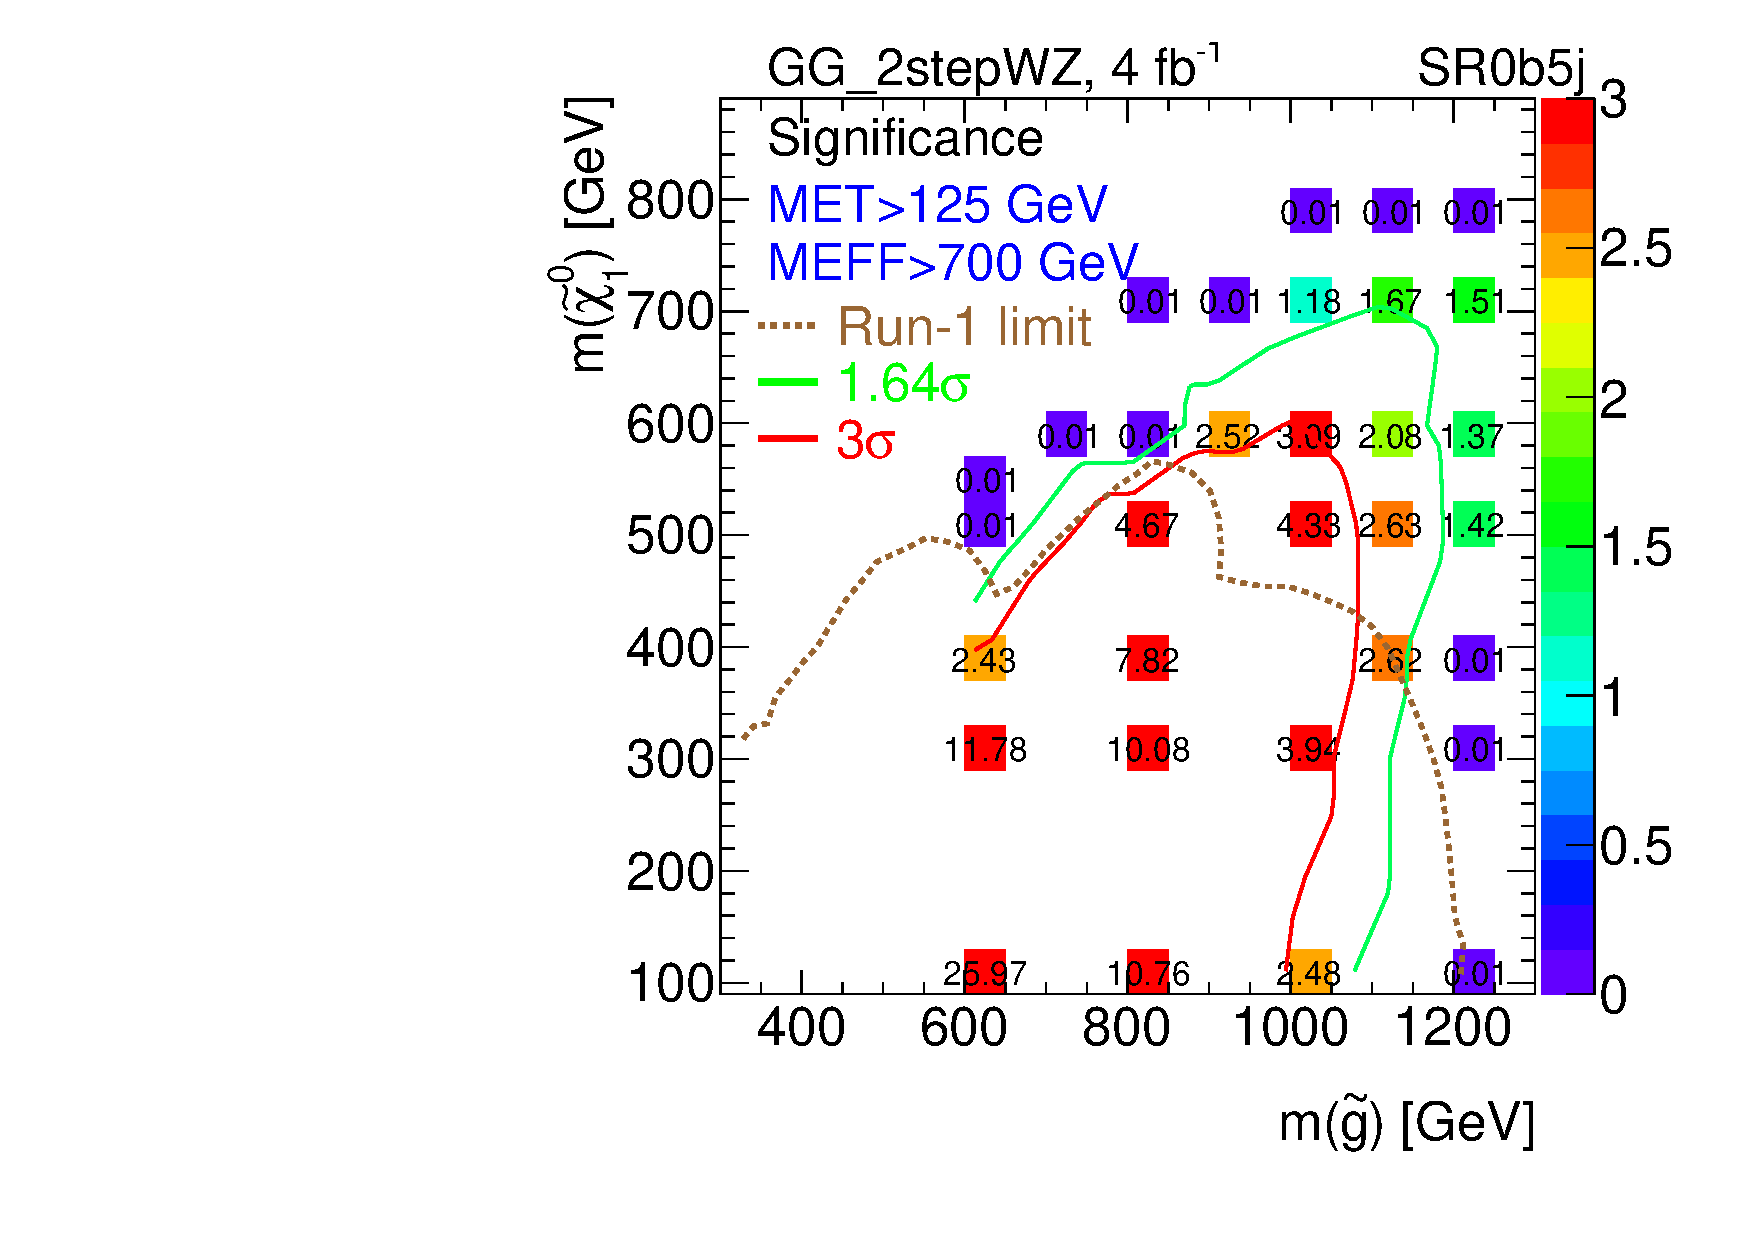
\includegraphics[width=0.4\textwidth]{OPTIMIZATION/Optimiz_SR0b5j_4fb_125_700.pdf}
  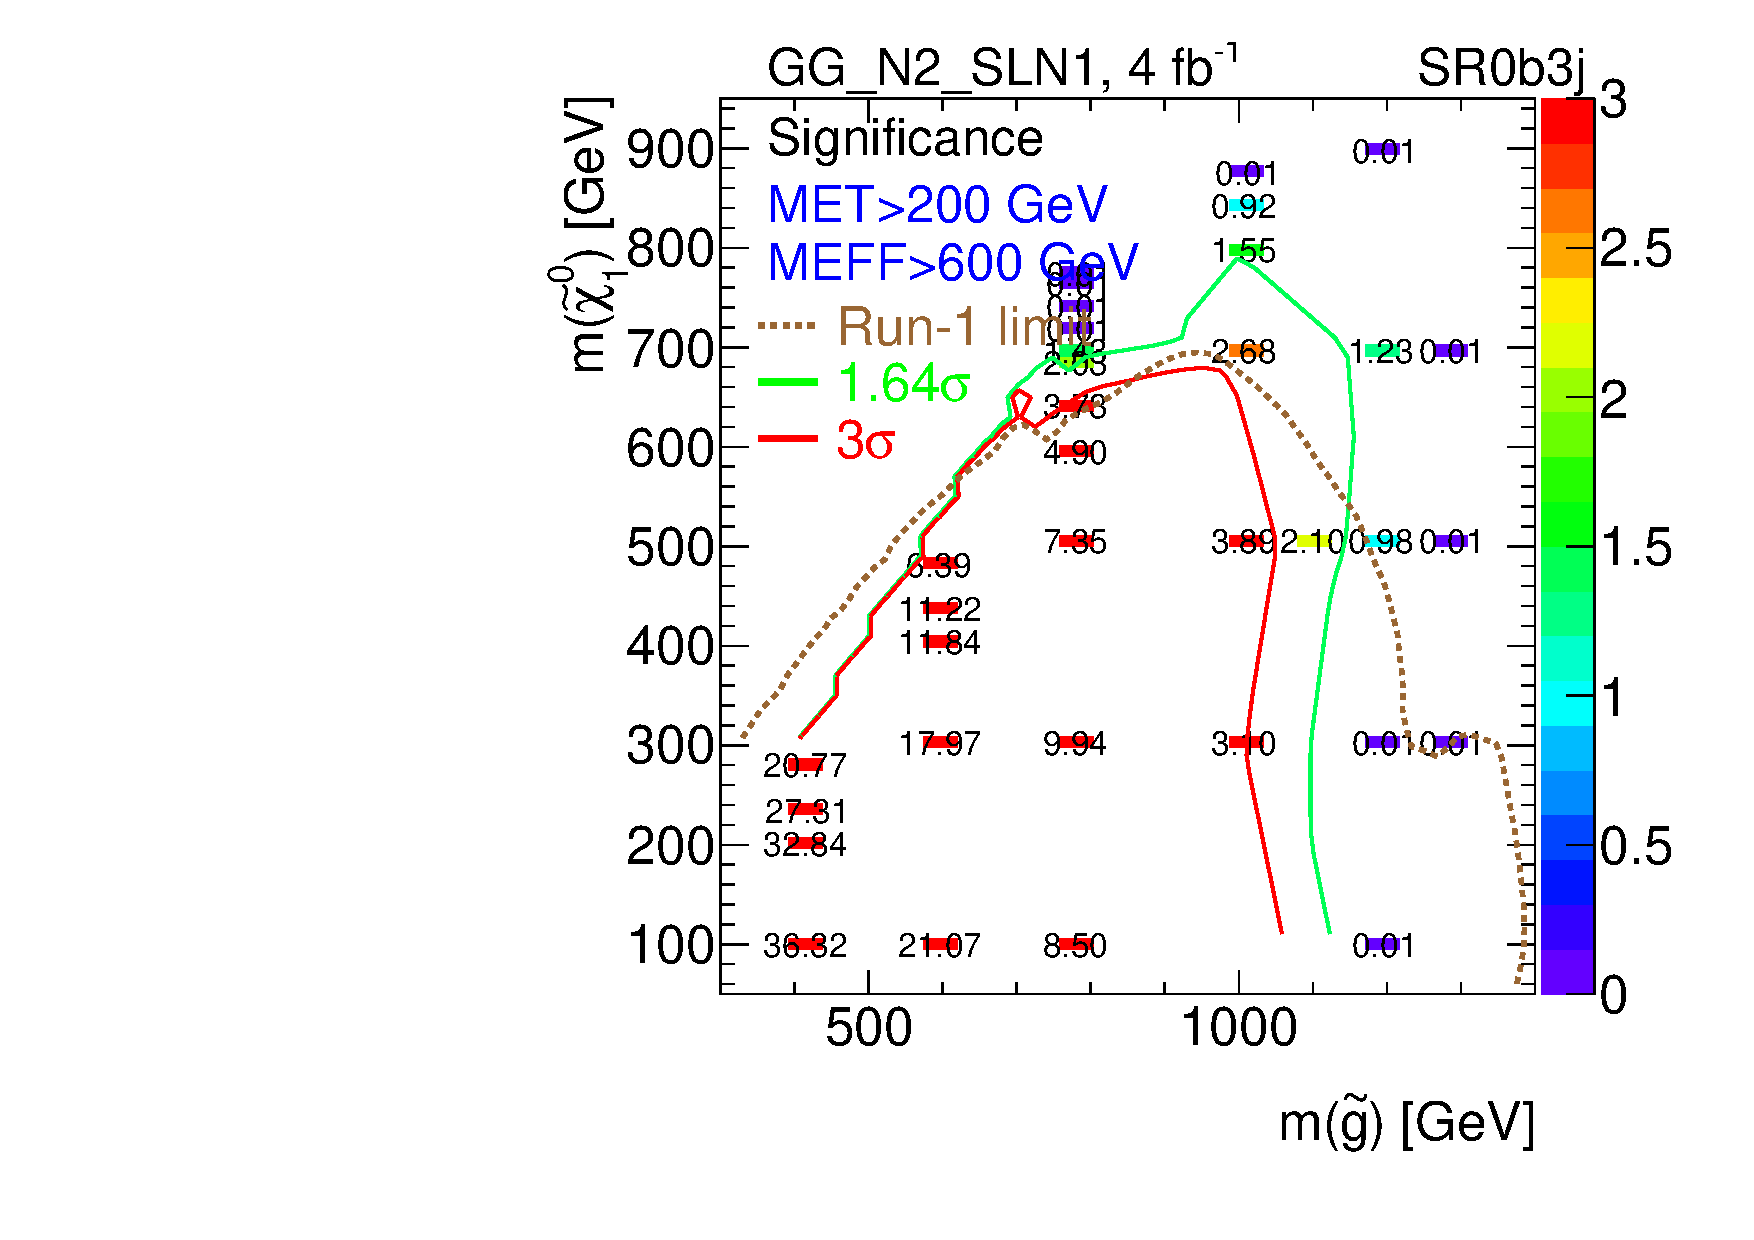
\includegraphics[width=0.4\textwidth]{OPTIMIZATION/Optimiz_SR0b3j_4fb_200_600.pdf}
  \caption{Discovery significance for the SRs defined in Table~\ref{tab:SRdef4} (4~\ifb) for SR1b in the $\sbot\sbot^*\to t\bar t\tilde\chi_1^+\tilde\chi_1^-$ grid (top left), SR3b in the $\gluino\gluino\to t\bar tt\bar t\ninoone\ninoone$ grid (top right), SR0b5j in the $\gluino\gluino$ with $\gluino\to q\bar{q}'WZ\ninoone$ grid (bottom left) and SR0b3j in the $\gluino\gluino$ with $\gluino\to q\bar{q}(\ell\ell/\ell\nu)\ninoone$ grid (bottom right). The Run-1 limits in those models are shown with a brown line, and the 1.64$\sigma$ and 3$\sigma$ discovery contours from the proposed signal regions are shown in green and red, respectively.}
\label{fig:OptimSig4}
\end{figure}


%\FloatBarrier
